\documentclass[12pt,a4paper,twoside,openright]{report}
\let\openright=\cleardoublepage



%%% Choose a language %%%

\newif\ifEN
% \ENtrue   % uncomment this for english
\ENfalse   % uncomment this for czech

%%% Configuration of the title page %%%

\def\ThesisTitleStyle{mff} % MFF style
%\def\ThesisTitleStyle{cuni} % uncomment for old-style with cuni.cz logo
%\def\ThesisTitleStyle{natur} % uncomment for nature faculty logo

\def\UKFaculty{Faculty of Mathematics and Physics}
%\def\UKFaculty{Faculty of Science}

\def\UKName{Charles University in Prague} % this is not used in the "mff" style

% Thesis type names, as used in several places in the title
\def\ThesisTypeTitle{\ifEN BACHELOR THESIS \else BAKALÁŘSKÁ PRÁCE \fi}
%\def\ThesisTypeTitle{\ifEN MASTER THESIS \else DIPLOMOVÁ PRÁCE \fi}
%\def\ThesisTypeTitle{\ifEN RIGOROUS THESIS \else RIGORÓZNÍ PRÁCE \fi}
%\def\ThesisTypeTitle{\ifEN DOCTORAL THESIS \else DISERTAČNÍ PRÁCE \fi}
\def\ThesisGenitive{\ifEN bachelor \else bakalářské \fi}
%\def\ThesisGenitive{\ifEN master \else diplomové \fi}
%\def\ThesisGenitive{\ifEN rigorous \else rigorózní \fi}
%\def\ThesisGenitive{\ifEN doctoral \else disertační \fi}
\def\ThesisAccusative{\ifEN bachelor \else bakalářskou \fi}
%\def\ThesisAccusative{\ifEN master \else diplomovou \fi}
%\def\ThesisAccusative{\ifEN rigorous \else rigorózní \fi}
%\def\ThesisAccusative{\ifEN doctoral \else disertační \fi}



%%% Fill in your details %%%

% (Note: \xxx is a "ToDo label" which makes the unfilled visible. Remove it.)
\def\ThesisTitle{Nástroj pro průzkum a vizualizaci modelu pro simulátor mozku Mozaik}
\def\ThesisAuthor{Filip Ježek}
\def\YearSubmitted{2023}

% department assigned to the thesis
\def\Department{Katedra softwaru a výuky informatiky}
% Is it a department (katedra), or an institute (ústav)?
\def\DeptType{Katedra}

\def\Supervisor{Mgr. Ján Antolík, Ph.D.}
\def\SupervisorsDepartment{Katedra softwaru a výuky informatiky}

% Study programme and specialization
\def\StudyProgramme{Informatika}
\def\StudyBranch{Databáze a web}

\def\Dedication{%
  Rád bych poděkoval Mgr. Jánu Antolíkovi, Ph.D. za vedení této práce, za jeho čas a hodnotné rady. Dále bych rád poděkoval Rémy Cagnolovi a Tiboru Rózsovi z CSNG za výborné připomínky a podporu při vývoji. Rád bych také poděkoval své rodině a kamarádům.
}

\def\AbstractEN{%
  Simulations of biological neural networks are an important tool for understanding how the brain processes information. Mozaik is a workflow framework that allows such simulations to be created, run and analyzed. Currently, however, there is no easy way to visualize in it either the network or the data structures created by individual analyses. This work is a web application that allows users to visualize networks and data structures stored in datastores for individual simulations. The given visualizations can be searched using complex queries, interactively examined and compared with each other. This makes the work of researchers working with the Mozaik framework much more efficient.
  % ABSTRACT IS NOT A COPY OF YOUR THESIS ASSIGNMENT!
}

\def\AbstractCS{%
  Simulace biologických neuronových sítí jsou důležitým nástrojem pro porozumění tomu, jak mozek zpracovává informace. Mozaik je workflow framework, který umožňuje takové simulace vytvářet, spouštět a analyzovat. V~současné době ale neexistuje snadný způsob, jak v~něm vizualizovat ani síť, ani datové struktury vytvořené jednotlivými analýzami. Tato práce je webová aplikace, která umožňuje vizualizovat sítě a~datové struktury uložené v datastorech pro jednotlivé simulace. Dané vizualizace lze vyhledávat pomocí komplexních dotazů, interaktivně je zkoumat a~vzájemně mezi sebou srovnávat. To výrazně zefektivňuje práci výzkumníků, kteří s~frameworkem Mozaik zacházejí.
}

% 3 to 5 keywords (recommended), each enclosed in curly braces.
% Keywords are useful for indexing and searching for the theses by topic.
\def\Keywords{%
  {vizualizace} {webová aplikace} {vědecký software} {biologické neuronové sítě} {neurověda}
}

% If your abstracts are long and do not fit in the infopage, you can make the
% fonts a bit smaller by this setting. (Also, you should try to compress your abstract more.)
% Alternatively, consider increasing the size of the page by uncommenting the
% geometry modification in thesis.tex.
\def\InfoPageFont{}
%\def\InfoPageFont{\small}  %uncomment to decrease font size

\ifEN\relax\else
  % If you are writing a czech thesis, you additionally need to fill in the
  % english translation of the metadata here!
  \def\ThesisTitleEN{A model inspection/visualization tool for brain simulation framework}
  \def\DepartmentEN{Department of Software and Computer Science Education}
  \def\DeptTypeEN{Department}
  \def\SupervisorsDepartmentEN{Department of Software and Computer Science Education}
  \def\StudyProgrammeEN{Computer Science}
  \def\StudyBranchEN{Databases and Web}
  \def\KeywordsEN{%
    {visualization} {web application} {scientific software} {biological neural networks} {neuroscience}
  }
  
\fi


\usepackage[a-2u]{pdfx}

\ifEN\else\usepackage[czech,shorthands=off]{babel}\fi
\usepackage[utf8]{inputenc}
\usepackage[T1]{fontenc}

% See https://en.wikipedia.org/wiki/Canons_of_page_construction before
% modifying the size of printable area. LaTeX defaults are great.
% If you feel it would help anything, you can enlarge the printable area a bit:
\usepackage[textwidth=390pt,textheight=630pt]{geometry}
% The official recommendation expands the area quite a bit (looks pretty harsh):
%\usepackage[textwidth=145mm,textheight=247mm]{geometry}

%%% FONTS %%%
\usepackage{lmodern} % TeX "original" (this sets up the latin mono)

% Optionally choose an override for the main font for typesetting:
\usepackage[mono=false]{libertinus} % popular for comp-sci (ACM uses this)
%\usepackage{tgschola} % Schoolbook-like (gives a bit of historic feel)
%\usepackage[scale=0.96]{tgpagella} % Palladio-like (popular in formal logic).
% IBM Plex font suite is nice but requires us to fine-tune the sizes, also note
% that it does not directly support small caps (\textsc) and requires lualatex:
%\usepackage[usefilenames,RM={Scale=0.88},SS={Scale=0.88},SScon={Scale=0.88},TT={Scale=0.88},DefaultFeatures={Ligatures=Common}]{plex-otf}

% Optionally, choose a custom sans-serif fonts (e.g. for figures and tables).
% Default sans-serif font is usually Latin Modern Sans. Some font packages
% (e.g. libertinus) replace that with a better matching sans-serif font.
%\usepackage{tgheros} % recommended and very readable (Helvetica-like)
%\usepackage{FiraSans} % looks great
% DO NOT typeset the main text in sans-serif font!
% The serifs make the text easily readable on the paper.


% IMPORTANT FONT NOTE: Some fonts require additional PDF/A conversion using
% the pdfa.sh script. These currently include only 'tgpagella'; but various
% other fonts from the texlive distribution need that too (mainly the Droid
% font family).


% some useful packages
\usepackage{microtype}
\usepackage{amsmath,amsfonts,amsthm,bm}
\usepackage{graphicx}
\usepackage{xcolor}
\usepackage{booktabs}
\usepackage{caption}
\usepackage{floatrow}
\usepackage{xurl}
\usepackage{pdfpages}

% load bibliography tools
\usepackage[backend=bibtex,natbib,style=numeric,sorting=none]{biblatex}
% alternative with alphanumeric citations (more informative than numbers):
%\usepackage[backend=bibtex,natbib,style=alphabetic]{biblatex}
%
% alternatives that conform to iso690
% (iso690 is not formally required on MFF, but may help elsewhere):
%\usepackage[backend=bibtex,natbib,style=iso-numeric,sorting=none]{biblatex}
%\usepackage[backend=bibtex,natbib,style=iso-alphabetic]{biblatex}
%
% additional option choices:
%  - add `giveninits=true` to typeset "E. A. Poe" instead of full Edgar Allan
%  - `terseinits=true` additionaly shortens it to nature-like "Poe EA"
%  - add `maxnames=10` to limit (or loosen) the maximum number of authors in
%    bibliography entry before shortening to `et al.` (useful when referring to
%    book collections that may have hundreds of authors)
%  - for additional flexibility (e.g. multiple reference sections, etc.),
%    remove `backend=bibtex` and compile with `biber` instead of `bibtex` (see
%    Makefile)
%  - `sorting=none` causes the bibliography list to be ordered by the order of
%    citation as they appear in the text, which is usually the desired behavior
%    with numeric citations. Additionally you can use a style like
%    `numeric-comp` that compresses the long lists of citations such as
%    [1,2,3,4,5,6,7,8] to simpler [1--8]. This is especially useful if you plan
%    to add tremendous amounts of citations, as usual in life sciences and
%    bioinformatics.
%  - if you don't like the "In:" appearing in the bibliography, use the
%    extended style (`ext-numeric` or `ext-alphabetic`), and add option
%    `articlein=false`.
%
% possibly reverse the names of the authors with the default styles:
%\DeclareNameAlias{default}{family-given}

% load the file with bibliography entries
\addbibresource{refs}

% remove this if you won't use fancy verbatim environments
\usepackage{fancyvrb}

% remove this if you won't typeset TikZ graphics
\usepackage{tikz}
\usetikzlibrary{positioning} %add libraries as needed (shapes, decorations, ...)

% remove this if you won't typeset any pseudocode
\usepackage{algpseudocode}
\usepackage{algorithm}

% remove this if you won't list any source code
\usepackage{listings}


\hypersetup{unicode}
\hypersetup{breaklinks=true}

\usepackage[noabbrev]{cleveref}


% various forms of TODOs (you should remove this before submitting)
\usepackage[textsize=tiny, backgroundcolor=yellow!25, linecolor=black!25]{todonotes}
\newcommand{\xxx}[1]{\textcolor{red!}{#1}}

 % remove this before compiling the final version


% use this for typesetting a chapter without a number, e.g. intro and outro
\def\chapwithtoc#1{\chapter*{#1}\addcontentsline{toc}{chapter}{#1}}

% If there is a line/figure overflowing into page margin, this will make the
% problem evident by drawing a thick black line at the overflowing spot. You
% should not disable this.
\overfullrule=3mm

% The maximum stretching of a space. Increasing this makes the text a bit more
% sloppy, but may prevent the overflows by moving words to next line.
\emergencystretch=1em

\ifEN
  \theoremstyle{plain}
  \newtheorem{thm}{Theorem}
  \newtheorem{lemma}[thm]{Lemma}
  \newtheorem{claim}[thm]{Claim}
  \newtheorem{defn}{Definition}
  \theoremstyle{remark}
  \newtheorem*{cor}{Corollary}
\else
  \theoremstyle{plain}
  \newtheorem{thm}{Věta}
  \newtheorem{lemma}{Lemma}
  \newtheorem{claim}{Tvrzení}
  \newtheorem{defn}{Definice}
  \newtheorem{exmp}{Příklad}
  \theoremstyle{remark}
  \newtheorem*{cor}{Důsledek}
  
\fi

\newenvironment{myproof}{
  \par\medskip\noindent
  \textit{\ifEN Proof \else Důkaz \fi}.
}{
  \newline
  \rightline{$\qedsymbol$}
}

% real/natural numbers
\newcommand{\R}{\mathbb{R}}
\newcommand{\N}{\mathbb{N}}

% asymptotic complexity
\newcommand{\asy}[1]{\mathcal{O}(#1)}

% listings and default lstlisting config (remove if unused)
\DeclareNewFloatType{listing}{}
\floatsetup[listing]{style=ruled}

\DeclareCaptionStyle{thesis}{style=base,font={small,sf},labelfont=bf,labelsep=quad}
\captionsetup{style=thesis}
\captionsetup[algorithm]{style=thesis,singlelinecheck=off}
\captionsetup[listing]{style=thesis,singlelinecheck=off}

% Customization of algorithmic environment (comment style)
\renewcommand{\algorithmiccomment}[1]{\textcolor{black!25}{\dotfill\sffamily\itshape#1}}

% Uncomment for table captions on top. This is sometimes recommended by the
% style guide, and even required for some publication types.
%\floatsetup[table]{capposition=top}
%
% (Opinionated rant:) Captions on top are not "compatible" with the general
% guideline that the tables should be formatted to be quickly visually
% comprehensible and *beautiful* in general (like figures), and that the table
% "head" row (with column names) should alone communicate most of the content
% and interpretation of the table. If you just need to show a long boring list
% of numbers (because you have to), either put some effort into showing the
% data in an attractive figure-table, or move the data to an attachment and
% refer to it, so that the boredom does not impact the main text flow.
%
% You can make the top-captions look much less ugly by aligning the widths of
% the caption and the table, with setting `framefit=yes`, as shown below.  This
% additionally requires some extra markup in your {table} environments; see the
% comments in the example table in `ch2.tex` for details.
%\floatsetup[table]{capposition=top,framefit=yes}

\ifEN\floatname{listing}{Listing}
\else\floatname{listing}{Výpis kódu}\fi
\lstset{ % use this to define styling for any other language
  language=Python,
  tabsize=2,
  showstringspaces=false,
  basicstyle=\footnotesize\tt\color{black!75},
  identifierstyle=\bfseries\color{black},
  commentstyle=\color{green!50!black},
  stringstyle=\color{red!50!black},
  keywordstyle=\color{blue!75!black}}

% Czech versions of the used cleveref references (It's not as convenient as in
% English because of declension, cleveref is limited to sg/pl nominative. Use
% plain \ref to dodge that.)
\ifEN\relax\else
  \crefname{chapter}{kapitola}{kapitoly}
  \Crefname{chapter}{Kapitola}{Kapitoly}
  \crefname{section}{sekce}{sekce}
  \Crefname{section}{Sekce}{Sekce}
  \crefname{subsection}{sekce}{sekce}
  \Crefname{subsection}{Sekce}{Sekce}
  \crefname{subsubsection}{sekce}{sekce}
  \Crefname{subsubsection}{Sekce}{Sekce}
  \crefname{figure}{obrázek}{obrázky}
  \Crefname{figure}{Obrázek}{Obrázky}
  \crefname{table}{tabulka}{tabulky}
  \Crefname{table}{Tabulka}{Tabulky}
  \crefname{listing}{výpis}{výpisy}
  \Crefname{listing}{Výpis}{Výpisy}
  \Crefname{appendix}{příloha}{přílohy}
  \Crefname{appendix}{Příloha}{Přílohy}
  \floatname{algorithm}{Algoritmus}
  \crefname{algorithm}{algoritmus}{algoritmy}
  \Crefname{algorithm}{Algoritmus}{Algoritmy}
  \newcommand{\crefpairconjunction}{ a~}
  \newcommand{\crefrangeconjunction}{ a~}
  
\fi
 % use this file for various custom definitions


\begin{document}

% the layout is mandatory, edit only in dire circumstances

\pagestyle{empty}
\hypersetup{pageanchor=false}
\begin{center}

% top part of the layout, this actually differs between faculties

\def\ThesisTitleXmff{%
  \ifEN
    \centerline{\mbox{
\includegraphics[width=166mm]{img/logo-en.pdf}}}
  \else
    \centerline{\mbox{
\includegraphics[width=166mm]{img/logo-cs.pdf}}}
  \fi
  \vspace{-8mm}\vfill%
  {\bf\Large\ThesisTypeTitle}
  \vfill%
  {\LARGE\ThesisAuthor}\par
  \vspace{15mm}%
  {\LARGE\bfseries\ThesisTitle}
  \vfill%
  \Department}
\def\ThesisTitleCuniLogo#1{%
  {\large\UKName\par\medskip\par\UKFaculty }
  \vfill%
  {\bf\Large\ThesisTypeTitle}
  \vfill%
  \includegraphics[width=70mm]{#1}
  \vfill%
  {\LARGE\ThesisAuthor}\par
  \vspace{15mm}%
  {\LARGE\bfseries\ThesisTitle}
  \vfill%
  \Department\par}
\def\ThesisTitleXcuni{\ThesisTitleCuniLogo{img/uklogo.pdf}}
\def\ThesisTitleXnatur{\ThesisTitleCuniLogo{img/naturlogo.pdf}}

% choose the correct page and print it
\csname ThesisTitleX\ThesisTitleStyle\endcsname
% latex corner: X is the new @

\vfill

{
\centerline{\vbox{\halign{\hbox to 0.45\hsize{\hfil #}&\hskip 0.5em\parbox[t]{0.45\hsize}{\raggedright #}\cr
\ifEN Supervisor of the \ThesisGenitive thesis:
\else Vedoucí \ThesisGenitive práce: \fi
& \Supervisor \cr
\noalign{\vspace{2mm}}
\ifEN Study programme: \else Studijní program: \fi
& \StudyProgramme \cr
\noalign{\vspace{2mm}}
\ifEN Study branch: \else Studijní obor: \fi
& \StudyBranch \cr
}}}}

\vfill

\ifEN Prague \else Praha \fi
\YearSubmitted

\end{center}

\newpage

% remember to sign this!
\openright
\hypersetup{pageanchor=true}
\pagestyle{plain}
\pagenumbering{roman}
\vglue 0pt plus 1fill

\ifEN
\noindent
I declare that I carried out this \ThesisAccusative thesis independently, and only with the cited
sources, literature and other professional sources. It has not been used to obtain another
or the same degree.
\else
\noindent
Prohlašuji, že jsem tuto \ThesisAccusative práci vypracoval(a) samostatně a výhradně
s~použitím citovaných pramenů, literatury a dalších odborných zdrojů.
Tato práce nebyla využita k získání jiného nebo stejného titulu.
\fi

\ifEN
\medskip\noindent
I understand that my work relates to the rights and obligations under the Act No.~121/2000 Sb.,
the Copyright Act, as amended, in particular the fact that the Charles
University has the right to conclude a license agreement on the use of this
work as a school work pursuant to Section 60 subsection 1 of the Copyright~Act.
\else
\medskip\noindent
Beru na~vědomí, že se na moji práci vztahují práva a povinnosti vyplývající
ze zákona č. 121/2000 Sb., autorského zákona v~platném znění, zejména skutečnost,
že Univerzita Karlova má právo na~uzavření licenční smlouvy o~užití této
práce jako školního díla podle §60 odst. 1 autorského zákona.
\fi

\vspace{10mm}


\ifEN
\hbox{\hbox to 0.5\hsize{%
In \hbox to 6em{\dotfill} date \hbox to 6em{\dotfill}
\hss}\hbox to 0.5\hsize{\dotfill\quad}}
\smallskip
\hbox{\hbox to 0.5\hsize{}\hbox to 0.5\hsize{\hfil Author's signature\hfil}}
\else
\hbox{\hbox to 0.5\hsize{%
V \hbox to 6em{\dotfill} dne \hbox to 6em{\dotfill}
\hss}\hbox to 0.5\hsize{\dotfill\quad}}
\smallskip
\hbox{\hbox to 0.5\hsize{}\hbox to 0.5\hsize{\hfil Podpis autora\hfil}}
\fi

\vspace{20mm}
\newpage

% dedication

\openright

\noindent
\Dedication

\newpage

% mandatory information page

\openright

\vbox to 0.49\vsize{\InfoPageFont
\setlength\parindent{0mm}
\setlength\parskip{5mm}

\ifEN Title: \else Název práce: \fi
\ThesisTitle

\ifEN Author: \else Autor: \fi
\ThesisAuthor

\DeptType:
\Department

\ifEN Supervisor: \else Vedoucí \ThesisGenitive práce: \fi
\Supervisor, \SupervisorsDepartment

\ifEN Abstract: \AbstractEN \else Abstrakt: \AbstractCS \fi

\ifEN Keywords: \else Klíčová slova: \fi
\Keywords

\vss}\ifEN\relax\else\nobreak\vbox to 0.49\vsize{\InfoPageFont
\setlength\parindent{0mm}
\setlength\parskip{5mm}

Title:
\ThesisTitleEN

Author:
\ThesisAuthor

\DeptTypeEN:
\DepartmentEN

Supervisor:
\Supervisor, \SupervisorsDepartmentEN

Abstract:
\AbstractEN

Keywords:
\KeywordsEN

\vss}
\fi

\newpage

\openright
\pagestyle{plain}
\pagenumbering{arabic}
\setcounter{page}{1}


\tableofcontents


\chapwithtoc{Úvod}

Porozumění lidskému mozku je téma, které v posledním desetiletí nabylo ještě většího významu. Mluví se o něm jak v souvislosti s umělou inteligencí, tak s neuroprotetikami. Klíčovým přístupem k výzkumu se stává výpočetní neurověda --- simulace jednotlivých vrstev neuronů, které napodobují mozkovou strukturu a funkcionalitu. CSNG~(Computational Systems Neuroscience Group)\footnote{\url{https://csng.mff.cuni.cz/}} z Matematicko-fyzikální fakulty za tímto účelem aktivně vyvíjí nástroj Mozaik\footnote{\url{https://github.com/CSNG-MFF/mozaik}}. Mozaik umožňuje specifikovat, spustit a analyzovat simulace neuronových sítí, přičemž veškerá data z takové simulace se ukládají do \emph{datastore}. Během simulace typicky běží několik algoritmů za různých podmínek, každý algoritmus pak generuje jednu nebo více \emph{datových struktur}. Tyto datové struktury je možné načítat pomocí Pythonu a zkoumat např. v Jupyter noteboocích. Dosud ale není možnost nějak uživatelsky přívětivě vizualizovat strukturu neuronových vrstev a spojení, ani uceleně zobrazit a filtrovat všechny datové struktury.

\section*{Cíle}

Cílem této práce je návrh a implementace webové aplikace pro vizualizaci modelu a datových struktur vygenerovaných za běhu Mozaiku. Aplikace by měla poskytnout rozhraní pro dotazy nad metadaty datových struktur, každý druh datové struktury by měl mít vlastní typ vizualizace a vizualizace by měly být interaktivní. Velká část práce s výsledky analýz je komparační, v aplikaci by tedy mělo být snadné porovnávat datové struktury vytvořené s různými parametry.

\section*{Struktura práce}

Nejprve si v kapitole \ref{chap:mozaik} přiblížíme Mozaik. Podíváme se na základy práce s ním, ale hlavně se seznámíme se strukturou datastore, ze kterého budeme získávat data. Také je důležité popsat návaznost na předchozí práce v tomto směru. V kapitole \ref{chap:requirements} formulujeme přesné požadavky na aplikaci. Kapitola \ref{chap:architecture} bude věnována popisu architektury, jejíž implementaci pak rozvedeme v kapitole \ref{chap:implementation}. Speciálně se podíváme na klíčové třídy frontendu v kapitole \ref{chap:frontend}. Posléze si v kapitole \ref{chap:howto} přiblížíme zacházení s programem. Konečně v příloze \ref{app:api} je podrobně popsáno serverové API.

\chapter{Mozaik}
\label{chap:mozaik}
\section{Práce s frameworkem}

Mozaik je framework pro Python, pomocí kterého lze snadno specifikovat 2-rozměrné vrstvy neuronů, nad kterými pak běží experimenty. Experimenty produkují data, která lze analyzovat různými algoritmy a~zaznamenávat jejich výstupy. V Mozaik tutorialu\cite{MozaikTutorial} je ukázán příklad, na který se zde (v~trochu zkrácené podobě) podíváme.

\begin{figure}
  \centering
  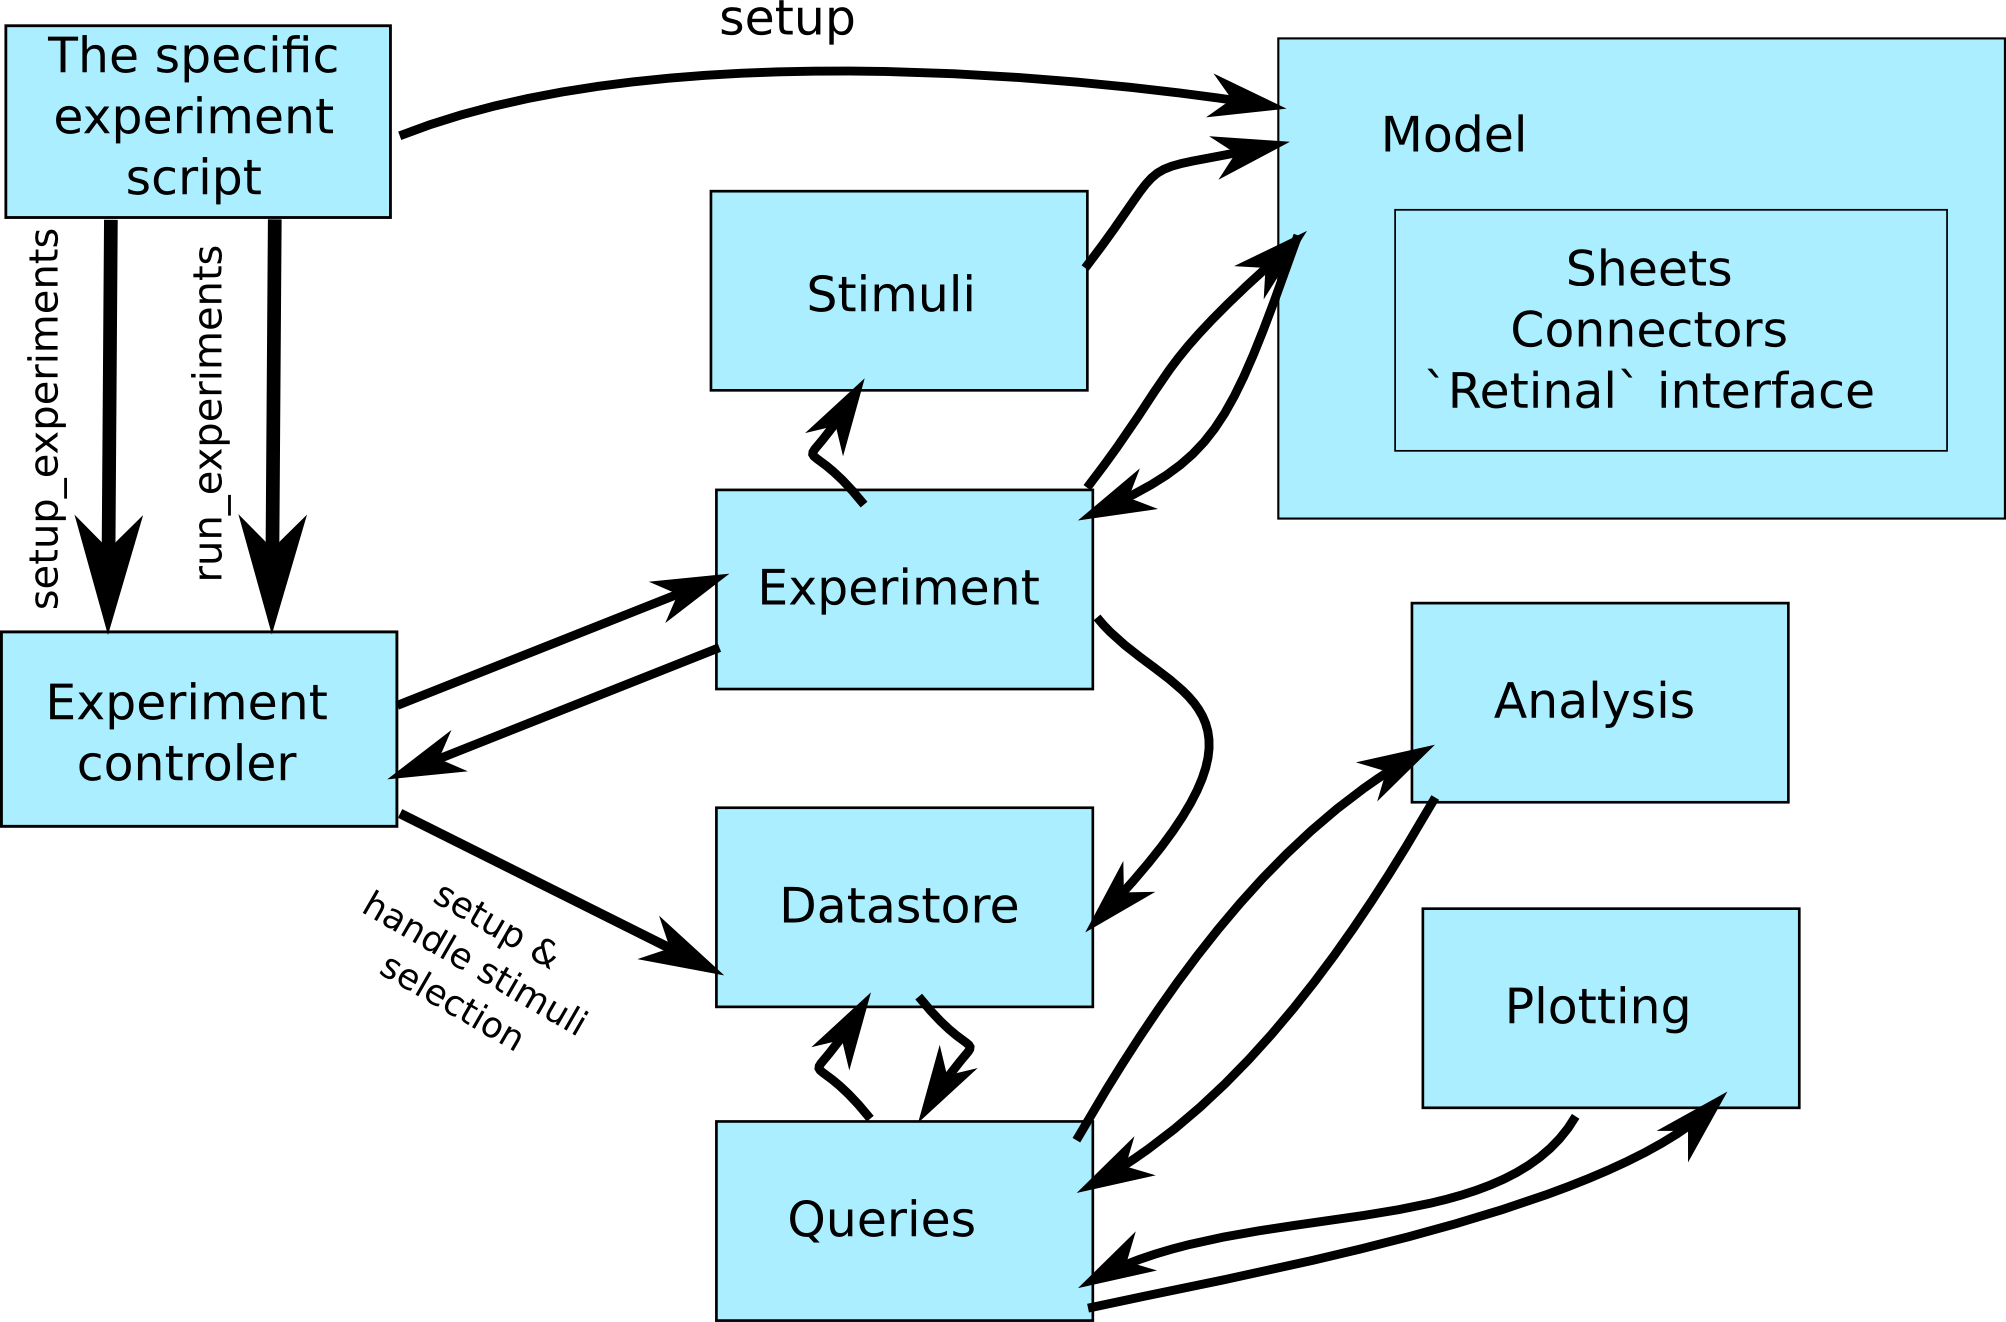
\includegraphics[width=.6\linewidth]{img/mozaik_control_flow.png}
  \caption{Control flow mezi jednotlivými komponentami Mozaiku\cite{MozaikIntroduction}}
\end{figure}

Kód je rozdělen na 6~hlavních částí. Část 1 a~2 jsou definice neuronových vrstev --- třída \lstinline|Model| a~její parametry. Stejný neuron může být součástí více vrstev na různých souřadnicích.

\begin{lstlisting}[language=Python]
  class VogelsAbbott( Model ):
    # parametry jsou nacteny z oddeleneho souboru
    required_parameters = ParameterSet({
      # definujeme 2 neuronove vrstvy
      'sheets': ParameterSet({
          'exc_layer': ParameterSet,
          'inh_layer': ParameterSet, 
      })
    })

    def __init__(self, sim, num_threads, parameters):
      Model.__init__(self, sim, num_threads, parameters)
      # nacteni komponent vrstev
      ExcLayer = load_component(
        self.parameters.sheets.exc_layer.component
      )
      ...
      
      exc = ExcLayer(
        self, 
        self.parameters.sheets.exc_layer.params
      )
      ...

      # spojeni mezi vrstvami
      UniformProbabilisticArborization(
        self,'ExcExcConnection',exc,exc,
        self.parameters.sheets.exc_layer.ExcExcConnection
      ).connect()
      ...
\end{lstlisting}

Dále je potřeba specifikovat samotné experimenty, které chceme na mozku provést.

\begin{lstlisting}[language=Python]
def create_experiments(model):
  return [
    #Lets kick the network up into activation
    PoissonNetworkKick(model,ParameterSet({
      'duration': 8*7,
      'drive_period': 8*7.0,
      'sheet_list': ["Exc_Layer","Inh_Layer"],
      'stimulation_configuration' : {
        'component':
          'mozaik.sheets.population_selector'
          '.RCRandomPercentage',
        'params': {'percentage' : 20.0}
      },
      'lambda_list': [100.0,100.0],
      'weight_list': [0.1,0.1]
    })),
    #Spontaneous Activity 
    NoStimulation(model,ParameterSet({'duration': 135.0*2}))
  ]
\end{lstlisting}

Experimenty produkují surová data, \emph{segmenty}. Ta nám sama o sobě moc neřeknou, ale můžeme na nich spouštět analytické algoritmy. Ještě předtím ale spustíme samotnou simulaci.

\begin{lstlisting}[language=Python]
data_store,model = run_workflow(
  'example simulation',
  VogelsAbbott,
  create_experiments
)
\end{lstlisting}

Segmenty jsou uložené v datastore a nám už nic nebrání je analyzovat.

\begin{lstlisting}[language=Python]
def perform_analysis_and_visualization(data_store):
  analog_ids = sorted(
    param_filter_query(data_store,sheet_name="Exc_Layer") \
    .get_segments()[0].get_stored_esyn_ids()
  )
  ...

  
  PopulationMeanAndVar(
    data_store,ParameterSet({'ignore_nan_and_inf': False})
  ).analyse()
  ...
\end{lstlisting}

V tuto chvíli můžeme použít modul \lstinline|mozaik.visualization| a vygenerovat množství rozmanitých grafů, které se uloží jako png soubory. My ale tuto funkcionalitu používat nebudeme a podíváme se raději na různé typy datových struktur, které se v datastore mohou nacházet.

\section{Datastore}

Datastore se na disk serializuje ve formátu pickle, což je binární protokol pro serializaci python objektů. Kromě \emph{ADS}~(analysis data structure) se v něm nachází metadata o neuronech, jejich vrstvách a stimulech. ADS lze vyhledávat pomocí jejich parametrů. ADS může být (ale nemusí) být spojena s konkrétní vrstvou, stimulem, nebo konkrétním neuronem. Dělí se na několik typů, podle typu dat, které uchovávají.

\subsection{SingleValue}

V celku triviální wrapper pro jedinou hodnotu.

\subsection{SingleValueList}

Jednorozměrný seznam hodnot.

\subsection{PerNeuronValue}

Podobná datová struktura jako SingleValueList, ale každá hodnota v seznamu odpovídá konkrétnímu neuronu.

\subsection{PerNeuronPairValue}

Seznam neuronů a matice hodnot pro každý jejich pár.

\subsection{AnalogSignal}

Jde o wrapper nad Neo \lstinline|AnalogSignal| \footnote{\url{https://neo.readthedocs.io/en/stable/api_reference.html\#neo.core.AnalogSignal}}, což je dvourozměrné pole periodicky měřených hodnot. Jedna dimenze odpovídá času a druhá jednotlivým zaznamenávaným kanálům. V praxi se ale v Mozaiku do AnalogSignalu zaznamenává pouze jeden kanál, takže se hodí o něm uvažovat jako o jednorozměrném poli.

\subsection{AnalogSignalList}

Kombinace PerNeuronValue a AnalogSignal. Seznam AnalogSignalů, kde každý AnalogSignal náleží specifickému neuronu.

\subsection{PerNeuronPairAnalogSignalList}

Tentokrát jde o kombinaci AnalogSignalu a PerNeuronPairValue. Seznam neuronů a matice AnalogSignalů pro každý jejich pár.

\subsection{ConductanceSignalList}

Jedná se o rozšířený AnalogSignalList s tím, že pro každý neuron jsou zde uloženy 2 AnalogSignaly.

\subsection{Connections}

Tato datová struktura popisuje spojení mezi neurony, což jsou orientované hrany v grafu. Každá hrana má navíc ještě specifikovanou váhu a zpoždění.

\section{Předchozí práce}

Tato práce navazuje na ročníkový projekt Kateřiny Čížkové~\cite{Cizkova2020nprg035}. Její program byla webová aplikace, která umožňovala interaktivně zobrazit neuronové vrstvy v~zadaném datastore. Původní záměr byl tento projekt rozšířit, ale, jak je v~dokumentaci projektu popsáno, kolegyně zvolila ne úplně vhodnou technologii a~doporučuje začít potenciálně zcela od začátku. Tato práce tedy namísto Python frameworku Bokeh používá Flask a~renderování vizualizací je specifikováno až ve frontendu (více podrobností je v~kapitole \ref{chap:implementation}). Podobnost kódu je naprosto minimální, nicméně zejména ze začátku sloužil jako výborná inspirace.
\chapter{Analýza požadavků}

Požadavky na aplikaci byly zadány dobře a~přesně, díky tomu, že vzešly přímo od budoucích uživatelů. Aplikace byla nasazena už během vývoje a~průběžně používána, což napomohlo najít nedostatky včas a~uvést ji do stávající podoby.

\section{Přenos velkého objemu dat}

Aplikace musí zvládnout načíst a~zpracovat datastory co největší velikosti. Velikost datastoru se pohybuje v~řádu gigabytů, neuronů mohou být desítky tisíc a~hran desítky milionů. Je potřeba minimalizovat velikost dat pro přenos po síti, a je důležité dát si pozor na nápor na paměť serveru. Výše zmíněná instance měla k dispozici zhruba 8G paměti --- na tento limit se během provozu alespoň ze začátku naráželo často. O něco méně je to problém u klienta. Pochopitelně se zdroji nechceme plýtvat, ale stroje, na kterých se aplikace ve výsledku spouští, patří výzkumníkům a jsou výkonné.

\section{Specifikace složek s datastore}

Datastore k prohlížení se nachází na straně serveru. Aplikaci lze spustit na lokálním počítači, nebo například na serveru se sdílenými adresáři více uživatelů. V obou případech se hodí zadat serveru cestu, odkud může začít procházat adresářový strom. Jednak aby se zrychlilo vyhledávání uživatele, jednak kvůli bezpečnosti v případě veřejně přístupného serveru. Aplikace nesmí akceptovat cestu k datastore, která by nebyla potomkem nakonfigurovaného kořene. Zároveň by mělo být možné specifikovat více kořenů naráz.

\section{Přehledný výpis ADS}

Aplikace je potřeba kvůli zrychlení práce uživatelů. ADS by měly být zobrazeny tak, aby se šlo co nejrychleji zorientovat a najít to, co uživatel chce. ADS mají mnoho stejných parametrů, ty je potřeba umět vyfiltrovat a zobrazit jen ty, ve kterých se liší.

\section{Filtrování a vyhledávání ADS}

Na předchozí požadavek navazuje nutnost mít kvalitní vyhledávací systém. ADS by mělo být možné snadno a intuitivně filtrovat a řadit. Zároveň musí být filtrovací systém dostatečně silný na to, aby zvládal i hodně komplikované dotazy. Filtry by měly být přizpůsobené jednotlivým datovým typům parametrů.

\section{Workspace s ADS}

Načítání konkrétní ADS ze serveru může zabrat netriviální množství času. Je nutné mít možnost některé ADS označit a udržovat je v paměti, aby mezi nimi bylo možné rychle přepínat. Zároveň je nutné mít možnost konkrétní ADS z paměti odstranit a uvolnit zdroje.

\section{Vícenásobné zobrazení}

V určitých případech je rušivé a zdržující muset pořád přepínat mezi několika ADS, obzvlášť pokud je uživatel srovnává a hledá rozdíly a podobnosti. Tehdy je potřeba umět zobrazit více ADS naráz vedle sebe.

\section{Sdílené nastavení}

Každý druh vizualizace má svá specifická nastavení. Někdy se hodí moci upravovat nastavení pro každou ADS zvlášť, ale v případě vícenásobného zobrazení musí existovat možnost upravovat nastavení pro všechny zobrazené vizualizace stejného typu naráz.

\section{Connections}

Aplikace musí umět zobrazit spojení mezi neurony ve stejné vrstvě. Vrstva by měla být vizualizována jako interaktivní scatterplot.

\section{PerNeuronValue}

Aplikace musí umět vizualizovat PerNeuronValue ADS. Vizualizace by měla mít stejnou podobu jako vizualizace Connections, ale neurony by měly mít přiřazenou barvu na základě své hodnoty.

\section{PerNeuronPairValue}

Aplikace musí umět vizualizovat PerNeuronValue ADS. Vizualizace by měla být maticový graf.

\section{AnalogSignalList}

Aplikace musí umět vizualizovat AnalogSignalList ADS.

\section{Udržovatelnost}

Jeden z nejdůležitějších požadavků je udržovatelnost aplikace. Aplikace musí být napsána srozumitelně a rozšiřitelně. Musí být použity moderní technologie, které pravděpodobně brzy nezaniknou. Aplikace musí být dokumentována a důkladně otestována automatickými testy.
\chapter{Návrh architektury}
\label{chap:architecture}

Aplikace se skládá ze dvou hlavních celků, webového klienta a serveru. Většina logiky je na straně klienta, server slouží pouze pro načítání dat z datastore.

\section{Server}

Server je minimální, chová se jako prostředník mezi datastore a klientem. Jeho součástí je modul pro souborový systém, pomocí něhož je možné procházet adresáře a vypisovat přítomné datastory. Model API načítá neurony v jednotlivých vrstvách a jejich spojení. ADS API pak načítá seznam a detaily datových struktur. Jak modelová část serveru, tak ADS část serveru kromě veřejného rozhraní zahrnují jen minimální transformaci dat do formátu vhodného pro frontend.

\begin{figure}
  \centering
  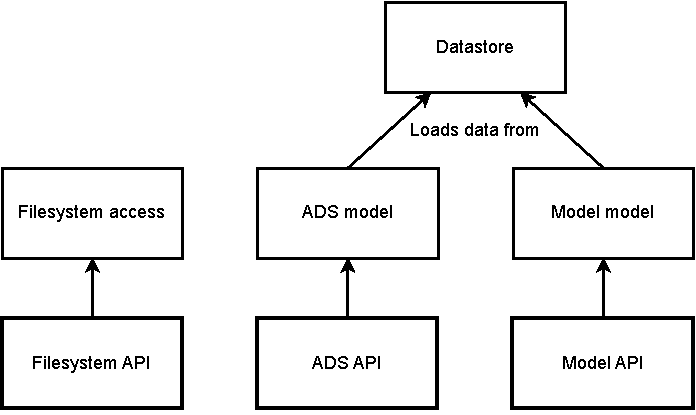
\includegraphics[width=.7\linewidth]{img/server_diagram.pdf}
  \caption{Architektura serveru}
\end{figure}

\subsection{Popis API}

Původní záměr byl vybudovat klasické JSON API. Během vývoje se ale ukázalo, že nejde o proveditelný nápad. Model i ADS zprávy mohou narůst do ohromné velikosti (například spojení mezi dvěma vrstvami mohou být desítky milionů). Když se server pokoušel zakódovat do JSON pole takových rozměrů, narazil na limit přidělené paměti. Jako JSON se tedy posílají jen relativně krátké zprávy, většinou metadata. Hlavní objem dat se streamuje ve formátu CSV. To má benefit i v lepším využití času na straně frontendu --- data se mohou začít zpracovávat už během stahování.

Speciální případ je načítání detailu ADS. Různé druhy ADS mají různě strukturovaná data s velkým objemem. Liší se jak dimenzionalita polí, tak jejich počet. API je vytvořené tak, aby frontend tyto informace nemusel předem znát. Detail API, který frontend dostane, místo některých properties může obsahovat \lstinline|@link| objekty. Ty frontendu sdělí, na jaké URI nalezne daná streamovaná data a jakou mají strukturu. Frontend si pak data automaticky nalezne sám. Rozměry CSV tabulky streamovaných ADS dat nemusí odpovídat rozměrům výsledného pole --- u více než dvourozměrného pole by to ani nebylo možné. Frontend si vytvoří prázdné pole správných rozměrů a do něj sekvenčně vyplňuje přijímaná data. Přidání nového druhu ADS tedy znamená změny v API pouze na straně serveru, načítací service v klientovi se měnit nemusí.

Trochu nešťastné je, že ADS nemají v datastore přiřazený žádný unikátní identifikátor. Jediný způsob, jak konkrétní ADS přesně popsat, je kombinace všech jejích základních atributů. Kvůli tomu některé metody v ADS API vyžadují netriviální množství parametrů, např. metoda pro načítání detailu ADS.

\begin{exmp}
  Uvažujme situaci, kdy frontend na svůj dotaz na konkrétní ADS dostane tuto odpověď.
  
  \begin{lstlisting}
    {
      type: 'PerNeuronPairValue',
      ids: [3, 4, 5],
      sheet: 'V1_Exc_L4',
      values: {
        '@link': '/ads/pnpv?path=datastore&sheet=V1_Exc_L4',
        dimensions: [3, 3]
      }
    }
  \end{lstlisting}
  
  Frontend v tuto chvíli musí získat data z poskytnuté cesty dalším dotazem. Pakliže server vygeneruje následující data:
  
  \begin{verbatim}
    16,7,8
    11,2,8
    22,9,1
  \end{verbatim}
  
  Výsledná ADS bude vypadat takto.
  
  \begin{lstlisting}
    {
      type: 'PerNeuronPairValue',
      ids: [3, 4, 5],
      sheet: 'V1_Exc_L4',
      values: [
        [16, 7, 8],
        [11, 2, 8],
        [22, 9, 1]
      ]
    }
  \end{lstlisting}
\end{exmp}

Podrobný popis celého API se nachází v příloze \ref{app:api}.

\section{Webový klient}

Klient sestává ze 4 hlavních vizuálních celků. Jedná se o souborový systém, navigátor, inspektor a přehled vybraných neuronů. Inspektor dále dynamicky instancuje modul pro vizualizaci v závislosti na typu vybrané ADS. Skutečná modulární struktura kódu silně vychází z použité technologie, proto bude podrobněji rozebrána v kapitole \ref{chap:implementation}.

Souborový systém, navigátor a inspektor představují postupně specifičtější pohledy do datastore. Při zcela čistém startu klienta je nutné jimi postupně projít, ale jejich stav se zároveň ukládá do URL, takže je možné některé kroky (za předpokladu poskytnutí správných hodnot v URL) při otevření webobé stránky přeskočit.

Protože při práci se občas hodí mít před očima co nejvíce informací naráz, a protože kvůli paměťové náročnosti není dobrý nápad mít aplikaci otevřenou naráz ve více záložkách prohlížeče, bylo potřeba najít způsob, jak umožnit změny layoutu a viditelnosti jednotlivých komponent. Zvolili jsme intuitivní způsob, na který už jsou uživatelé zvyklí z jiných míst. V klientovi jsou na několika místech použity kontejnery, zobrazující obsah vedle sebe, kde lze tažením myši měnit rozměry jednotlivých přihrádek. Ukázka na screenshotu \ref{fig:multiview}.

\begin{figure}
  \centering
  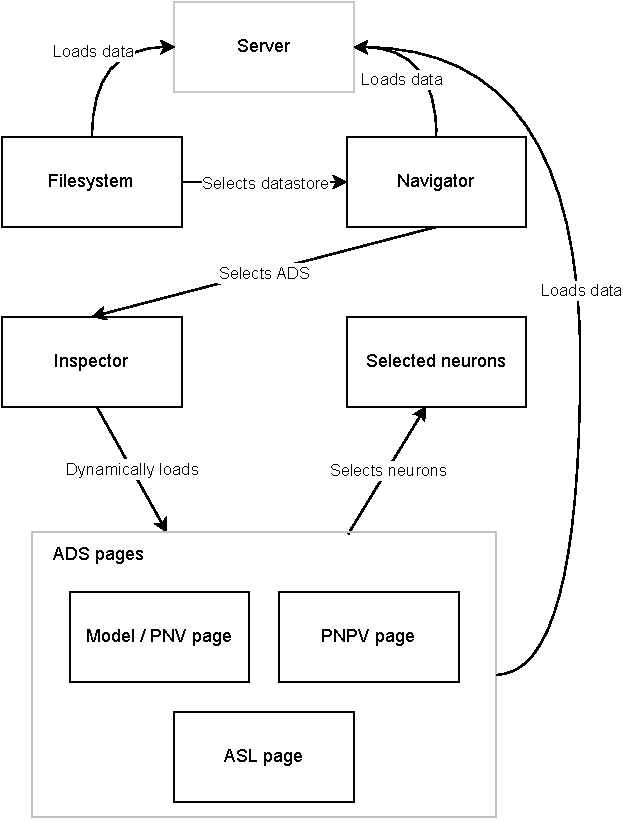
\includegraphics[width=.7\linewidth]{img/frontend_diagram.pdf}
  \caption{Architektura frontendu}
\end{figure}

\begin{figure}
  \centering
  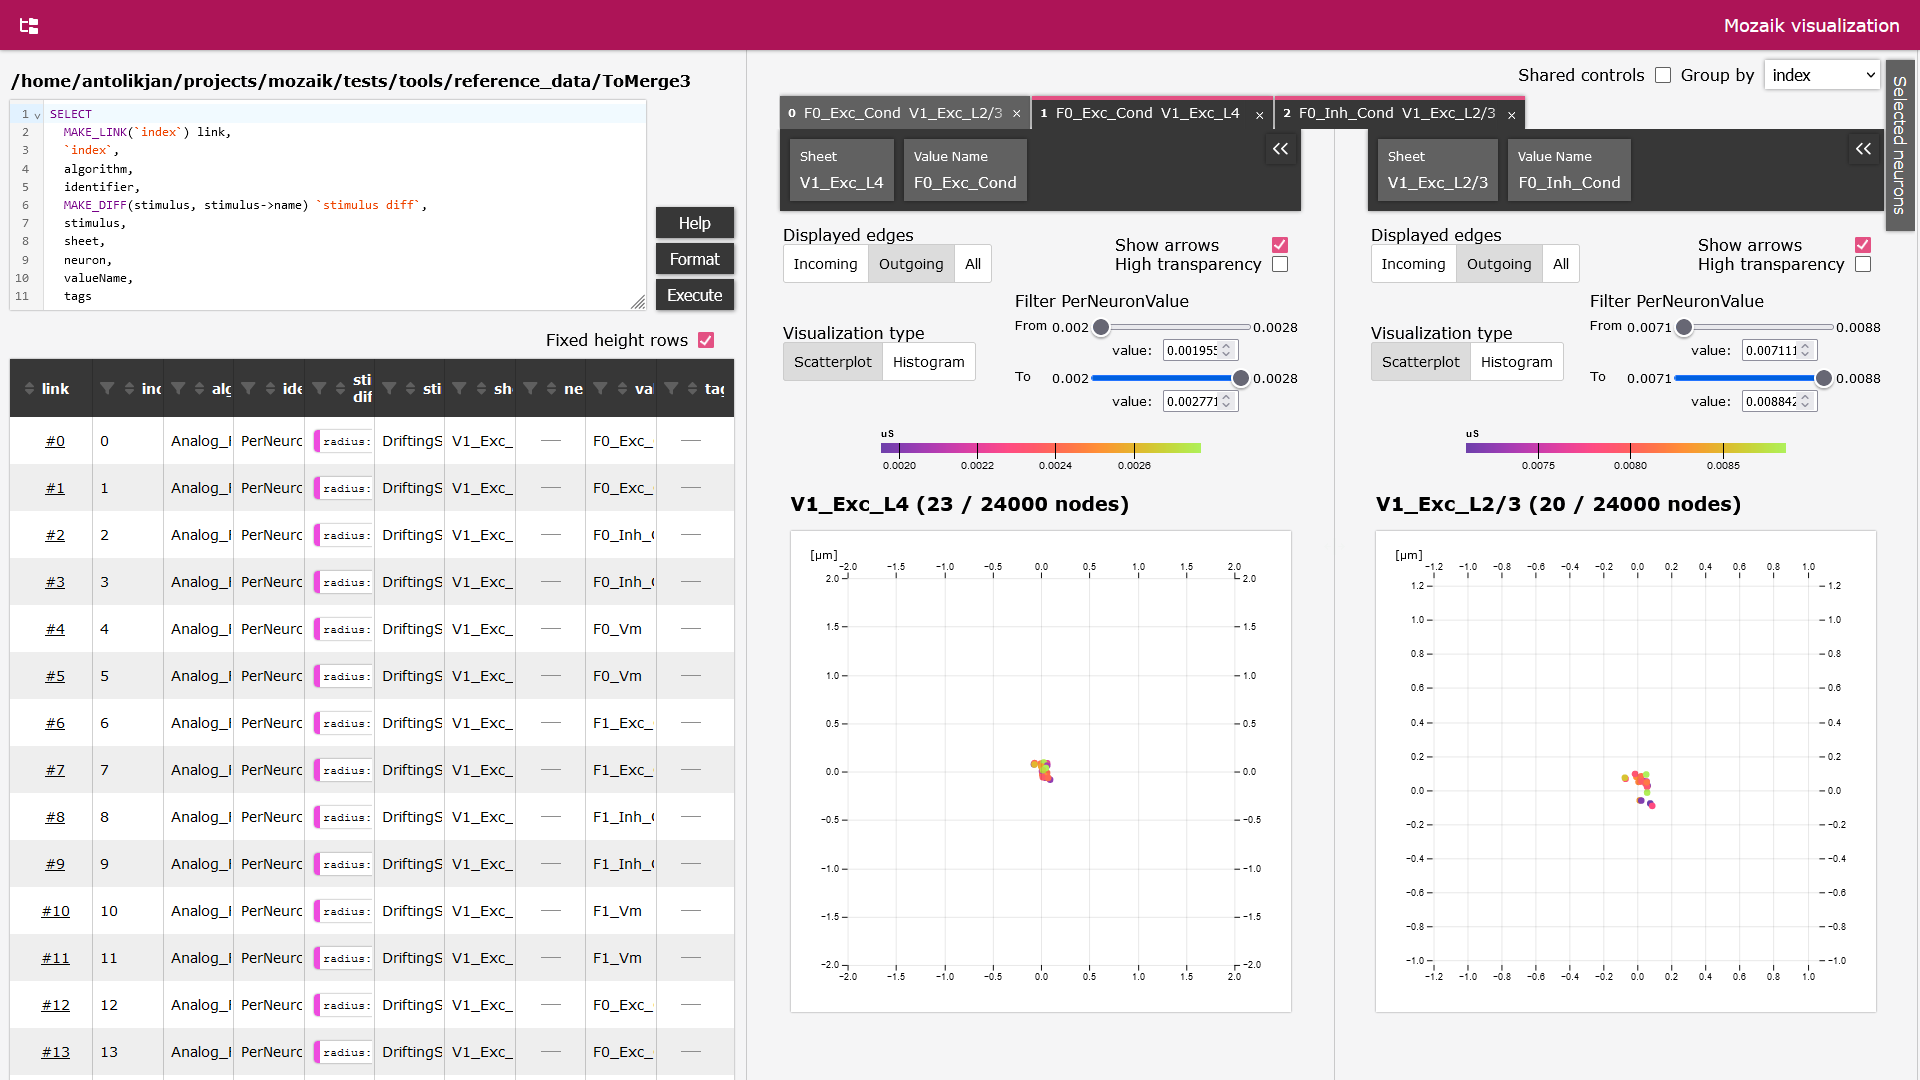
\includegraphics[width=1\linewidth]{img/screenshot_multiview.png}
  \caption{Ukázka upravovatelného layoutu. Na snímku lze vidět nalevo navigátor a napravo inspektor se dvěma aktuálně zobrazenými záložkami. Je možné myší tahat za hranici mezi navigátorem a inspektorem, za hranici mezi záložkami a za hranice mezi jednotlivými sloupci v navigátoru. Je také možné taháním za pravý okraj aplikace zobrazit sidebar s přehledem vybraných neuronů.}
  \label{fig:multiview}
\end{figure}

\subsection{Souborový systém}

Souborový systém zobrazuje složky a datastory. První složky, které uživatel uvidí, jsou nastaveny v konfiguraci a nelze se z nich dostat ven, pouze zanořovat dovnitř. Je možné rekurzivně prohledat celý adresářový strom a získat přehledně zobrazené pouze cesty, na kterých se nějaký datastore nachází. V určitých případech toto může být příliš pomalé, takže je tu ještě klasický způsob postupného zanořování se do složek. Jakmile uživatel zvolí zamýšlený datastore, klient načte základní data --- jednotlivé neuronové vrstvy a spojení a seznam všech ADS.

\subsection{Navigátor}

Navigátor reprezentuje tabulku ADS. Jednotlivé buňky obsahují různé datové typy parametrů, a musí tedy být specializované. Ve stejném sloupci se nicméně předpokládá stejný datový typ, podobně jako v relačních databázích. Jelikož je potřeba mít opravdu silný a robustní způsob vyhledávání, řazení a projekce ADS, je součástí navigátoru SQL editor. Je možné s ADS pracovat, jako by byly uloženy v relační tabulce s podporou pro datový typ JSON. Kromě standardního SQL jsme přidali několik dalších funkcí, které zjednodušují běžnou práci. Více se o nich opět lze dočíst v kapitole \ref{chap:implementation}. SQL jako součást user experience bylo zvolené s ohledem na to, že očekávanými uživateli jsou vývojáři. Pro zjednodušení ale byly přidány i klasické UX prvky. Sloupce lze jedním kliknutím řadit, lze je také filtrovat pomocí specializovaných dialogů. Interně jsou tyto akce nicméně opět převedeny na SQL query. Tyto pomocné filtry a řazení sice stačí po většinu času, na opravdu komplikované dotazy už ale je potřeba SQL měnit ručně.

\subsection{Inspektor}

Inspektor slouží k prohlížení jednotlivých vizualizací. Mezi požadavky na aplikaci je, že musí být možné vybrat několik ADS a mezi nimi rychle přepínat, nebo jich i zobrazit více vedle sebe. Na takovou činnost jsou uživatelé běžně zvyklí například z prohlížeče nebo textových editorů, které používají záložky. Inspektor proto pro co největší intuitivnost používá totéž řešení. Záložky lze řadit, otvírat, zavírat a kombinovat. Pro každou z nich se potom instancuje modul v závislosti na typu ADS. Za načítání doplňujících dat jsou pak zodpovědné právě tyto specializované moduly. 

\subsection{Přehled vybraných neuronů}

Jedná se o komponentu, která zobrazuje seznam právě vybraných neuronů a jejich metadata. Je možné zde výběr i zužovat či rozšiřovat.

\begin{figure}
  \centering
  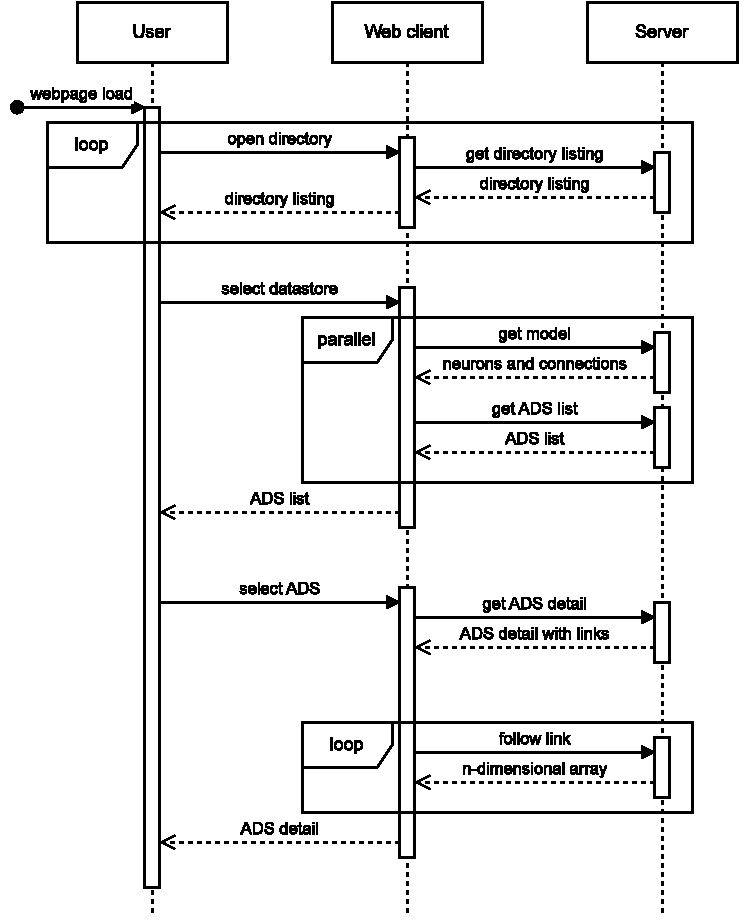
\includegraphics[width=.7\linewidth]{img/ads_sequence.pdf}
  \caption{Příklad komunikace webového klienta a serveru. Po spuštění aplikace je nejprve potřeba vybrat v adresářové struktuře správný datastore. Po jeho zvolení klient načte neuronové vrstvy a jejich spojení a seznam všech ADS. Uživatel si může některou z nich vybrat, tu pak klient načte pomocí jednoho až více dotazů a sestaví kompletní vizualizaci.}
\end{figure}


\chapwithtoc{Závěr}

Navrhli jsme a implementovali webovou aplikaci pro vizualizaci modelu a datových struktur vygenerovaných za běhu Mozaiku. Splnili jsme všechny vytyčené požadavky.

\begin{description}
  \item[Přenos velkého objemu dat] ze serveru je zajištěný streamováním ve formátu CSV. Je snadné část dat přenášených po síti ve formátu JSON začít také streamovat ve formátu CSV bez změny klienta.
  \item[Specifikace složek s datastore] je možná ve spouštěcím skriptu.
  \item[Přehledný výpis ADS] byl dosažen ve formě stránkované tabulky s buňkami specializovanými na různé datové typy.
  \item[Filtrování a vyhledávání ADS] je možné buď pomocí SQL, nebo pomocí dialogových oken.
  \item[Workspace s ADS] je implementováno ve formě záložek.
  \item[Vícenásobné zobrazení] je podporováno.
  \item[Sdílené nastavení] ADS je rovněž podporováno.
  \item[Connections] jsou vizualizovány jako interaktivní scatterplot.
  \item[PerNeuronValue] je vizualizována jako obarvený interaktivní scatterplot.
  \item[PerNeuronPairValue] je vizualizována jako interaktivní matice.
  \item[AnalogSignalList] je vizualizován jako interaktivní kombinace scatterplotu a čárového grafu.
  \item[Udržovatelnost] byla dosažena volbou frameworku, čistým a přehledným kódem a velkým množstvím automatických testů.
\end{description}

\section*{Možná rozšíření}

\subsection*{Alternativní barevné škály}

V různých případech se hodí použít různé barevné škály, v závislosti na tom, jaké informace jsou pro uživatele důležité a jak s daty chce zacházet\cite{silva2007there}. Zatím neexistuje v aplikaci možnost vybírat z jiných škál než z periodické a neperiodické. Tato funkčnost by přinesla možnost efektivnější analýzy.

\subsection*{Permutace maticové vizualizace}

Současná maticová vizualizace je užitečná pro rychlé zjištění specifické hodnoty. Je ale obtížné z ní vypozorovat existující trendy. Pro takovou funkčnost je nutné matici vhodně uspořádat\cite{chen2007handbook}. Bylo by vhodné implementovat jeden nebo více existujících algoritmů, například eliptickou seriaci\cite{chen2002generalized}

\ifEN
  \chapwithtoc{Bibliography}
\else
  \chapwithtoc{Seznam použitých zdrojů}

\fi

\printbibliography[heading=none]


\appendix
\chapter{Návod k použití}
\label{chap:howto}

\section{Instalace}

Nejprve je nutné nainstalovat runtime pro Python a Javascript.

\begin{itemize}
	\item Node.js 18
	\item Python 3.10
\end{itemize}

Pak je potřeba nainstalovat Mozaik. Přesný postup je uveden v jeho dokumentaci\cite{MozaikReadme}.

Dále doinstalujeme npm balíčky.

\begin{lstlisting}[language=bash]
	npm i -g @angular/cli
	cd frontend
	npm i
\end{lstlisting}

Ve stejné složce frontend zkompilujeme.

\begin{lstlisting}[language=bash]
	npm run build
\end{lstlisting}

\section{Spuštění}

Pro snadné spouštění je v kořenovém adresáři připraven skript \lstinline|run.sh|. Má několik volitelných parametrů.

\begin{lstlisting}[language=]
Start up flask server for mozaik visualization
Usage: ./run.sh [options]

Options:
		--expose
				listen on all network interfaces (default false)
		-h, --help
				display this message
		--port
				port to listen on (default 5000)
		--prod
				use production parameters (default false)
		--restart
				restart on crash (default false)
		--root
				root folder for looking up datastores,
				can be specified multiple times (default .)
\end{lstlisting}

\section{Testy}

Testy lze zvlášť spouštět pro Python a pro Angular.

\begin{lstlisting}[language=bash]
	pytest
	cd frontend
	npm run test
\end{lstlisting}

Angularové testy ze své podstaty musí běžet v prohlížeči. Adresa k otevření je vypsaná ve výstupu testovacího příkazu.

\section{Dev server}

Při vývoji Angularové části je doporučeno používat Angular dev server. Spustí se následujícím příkazem.

\begin{lstlisting}[language=bash]
	cd frontend
	npm run start
\end{lstlisting}

Tento server generuje sourcemaps pro snazší debugování, má zapnutou podporu pro store devtools, rekompiluje se při změnách kódu a automaticky přenačte otevřenou stránku. I nadále je ovšem potřeba mít spuštěný Flask server pro poskytnutí API.

\section{Základní práce s programem}

Protože program má grafické rozhraní, bylo by poněkud nešikovné bavit se o jeho používání jenom v textu. Následující část tedy bude sekvence obrázků, které nás provedou od načtení stránky po jednotlivé vizualizace. Aby byly dobře vidět, jsou některé screenshoty pořízeny na malé obrazovce. Při standardním běhu je na všechno více místa.

\begin{figure}
	\centering
	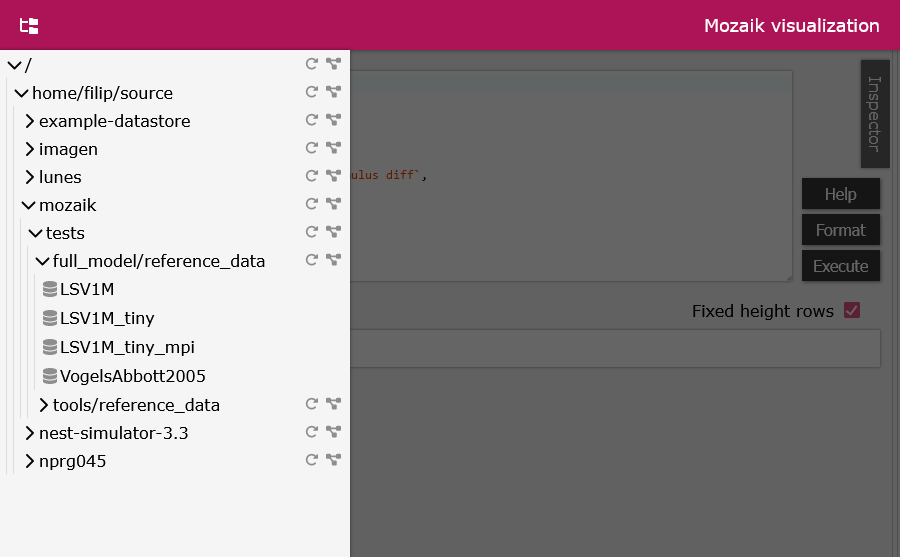
\includegraphics[width=1\linewidth]{img/screenshot_filesystem.png}
	\caption{Po načtení programu se zobrazí prohlížeč adresáře. Před další prací je nutno najít a vybrat datastore. Jednotlivé složky je možné procházet. Každá složka má navíc dvě tlačítka vpravo --- jedno z nich přenačte obsah složky a druhé její obsah načte rekurzivně a vyfiltruje složky bez datastore. Rekurzivně načtená byla složka \lstinline|mozaik|, proto jsou názvy některých složek v ní ve skutečnosti delší cesty.}
	\label{fig:filesystem}
\end{figure}

\begin{figure}
	\centering
	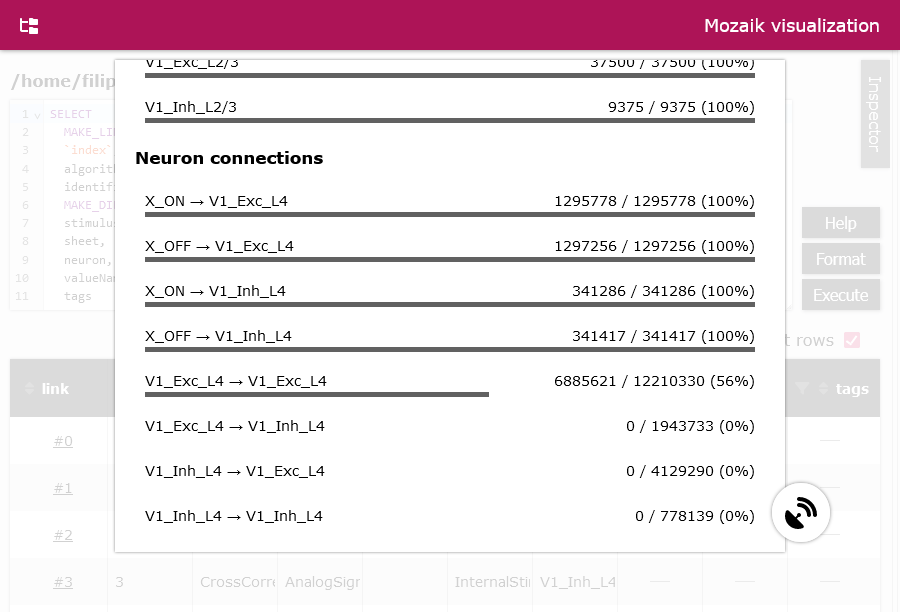
\includegraphics[width=1\linewidth]{img/screenshot_loading_model.png}
	\caption{Jakmile je datastore zvolen, načte se model. Při jeho načítání je vidět, kolik dat už se stáhlo. Vpravo dole je tlačítko, které zobrazí probíhající síťové dotazy --- to se zobrazí při jakékoli komunikaci po síti.}
	\label{fig:loading-model}
\end{figure}

\begin{figure}
	\centering
	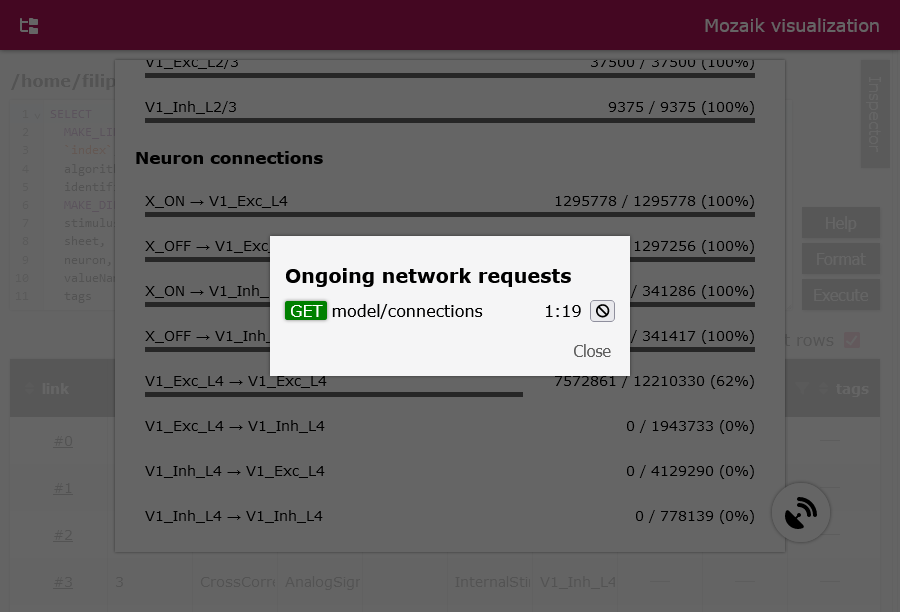
\includegraphics[width=1\linewidth]{img/screenshot_network.png}
	\caption{V tomto dialogu jsou vypsané jednotlivé probíhající dotazy. Dotaz může selhat a být spuštěn znovu, v takovém případě se zde ukazuje i o kolikátý pokus jde. Po kliknutí na tlačítko lze dotaz zrušit. To je vhodné v případě, že nejde o první pokus a dotaz zahrnuje hodně dat. Může to totiž znamenat, že byl server přetížen, došla mu paměť a byl mezitím restartován. Takový dotaz by akorát způsobil další restart serveru.}
	\label{fig:network}
\end{figure}

\begin{figure}
	\centering
	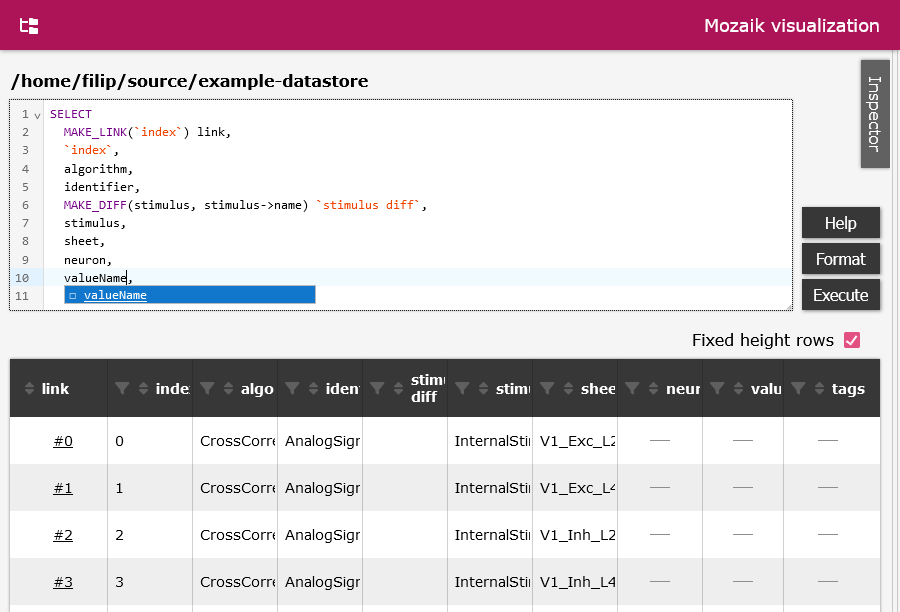
\includegraphics[width=1\linewidth]{img/screenshot_navigator.png}
	\caption{Všechny ADS jsou načteny do in-memory SQL tabulky, kterou je možné dotazovat. Po kliknutí na název sloupce je možné řádky seřadit. Vedle názvu je také vidět tlačítko pro zobrazení filtrů. V záhlaví celé stránky je nalevo vidět tlačítko pro otevření výběru datastore. To je dostupné neustále.}
	\label{fig:navigator}
\end{figure}

\begin{figure}
	\centering
	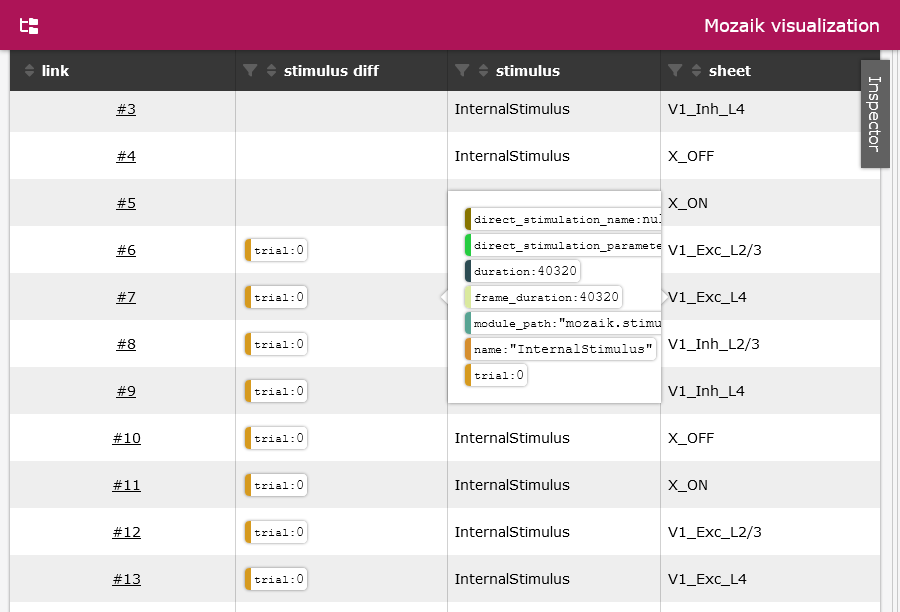
\includegraphics[width=1\linewidth]{img/screenshot_stimulus.png}
	\caption{Stimulus má většinou příliš mnoho parametrů na to, aby se do tabulky příjemně vešel. Zobrazuje se tedy jen jeho jméno a parametry jsou přístupné po najetí kurzorem.}
	\label{fig:stimulus}
\end{figure}

\begin{figure}
	\centering
	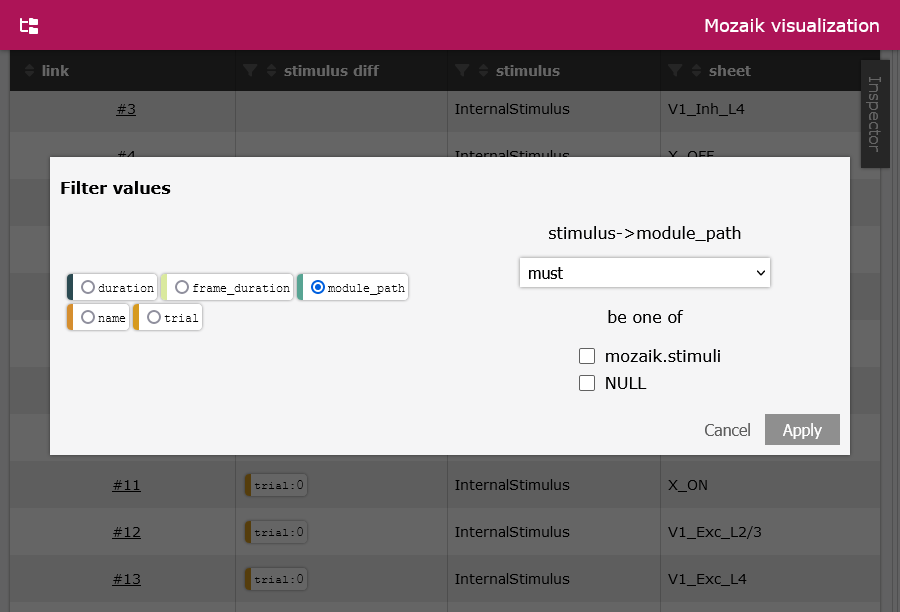
\includegraphics[width=1\linewidth]{img/screenshot_filter.png}
	\caption{Takto vypadá filtr sloupce s key-value hodnotami. Položka \lstinline|module_path| má mezi všemi stimuly jen dvě hodnoty, takže není třeba komplikovanějších podmínek.}
	\label{fig:filter}
\end{figure}

\begin{figure}
	\centering
	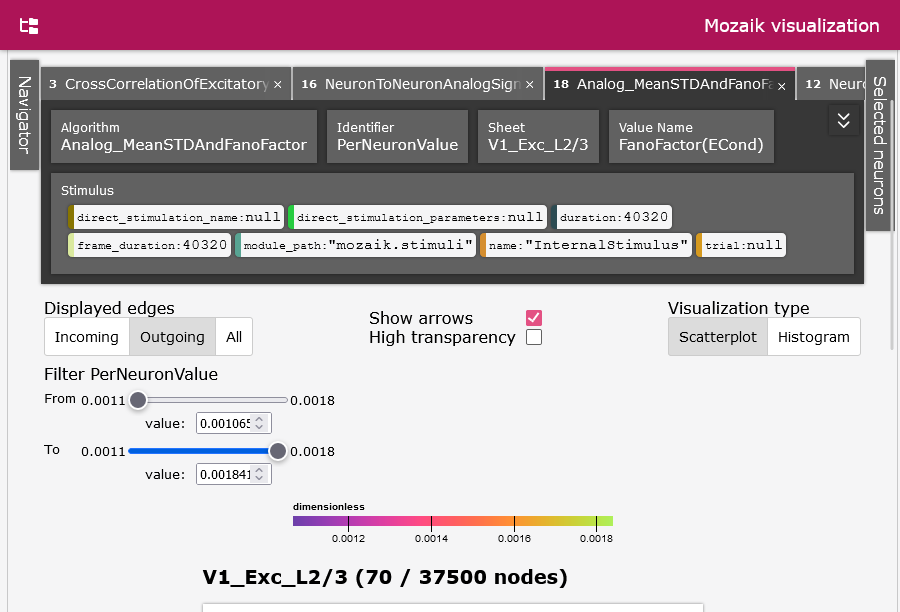
\includegraphics[width=1\linewidth]{img/screenshot_tabs.png}
	\caption{Takto vypadá inspektor jednotlivých ADS. Jména záložek jsou tvořena na základě odlišných parametrů.}
	\label{fig:tabs}
\end{figure}

\begin{figure}
	\centering
	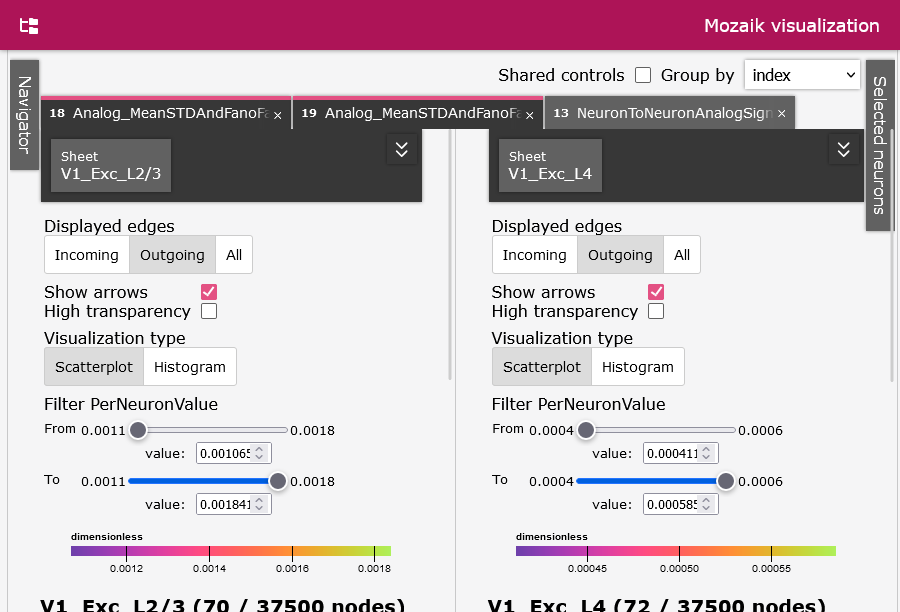
\includegraphics[width=1\linewidth]{img/screenshot_multiple_tabs.png}
	\caption{Když se vybere víc záložek naráz, základní informace o ADS ve tmavém bloku jsou redukovány na rozdílné položky.}
	\label{fig:multiple_tabs}
\end{figure}

\begin{figure}
	\centering
	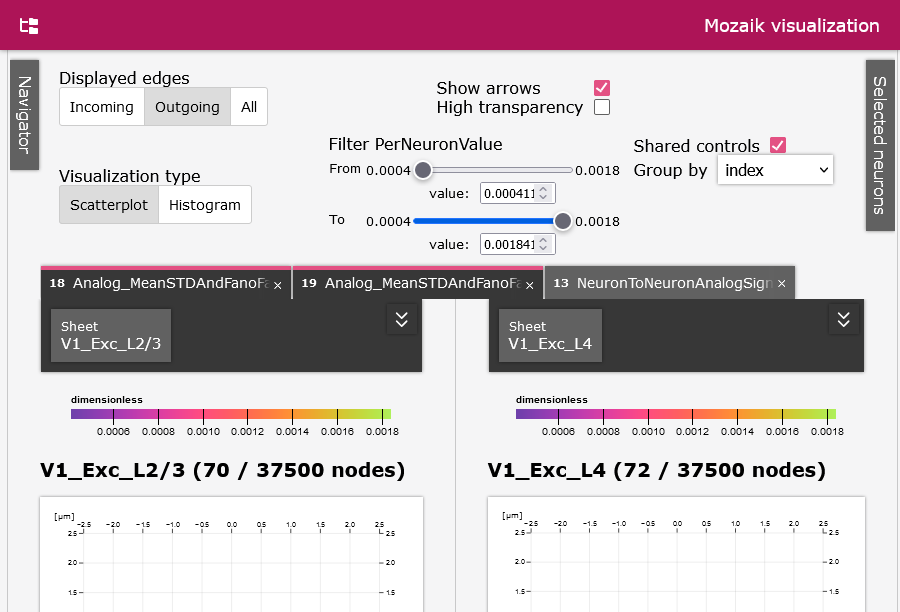
\includegraphics[width=1\linewidth]{img/screenshot_shared_controls.png}
	\caption{Když jsou sdílená nastavení záložek, přesouvají se nahoru. Je vidět, jak se oproti \ref{fig:multiple_tabs} propojilo minimum a maximum ve sliderech uprostřed.}
	\label{fig:shared_controls}
\end{figure}

\begin{figure}
	\centering
	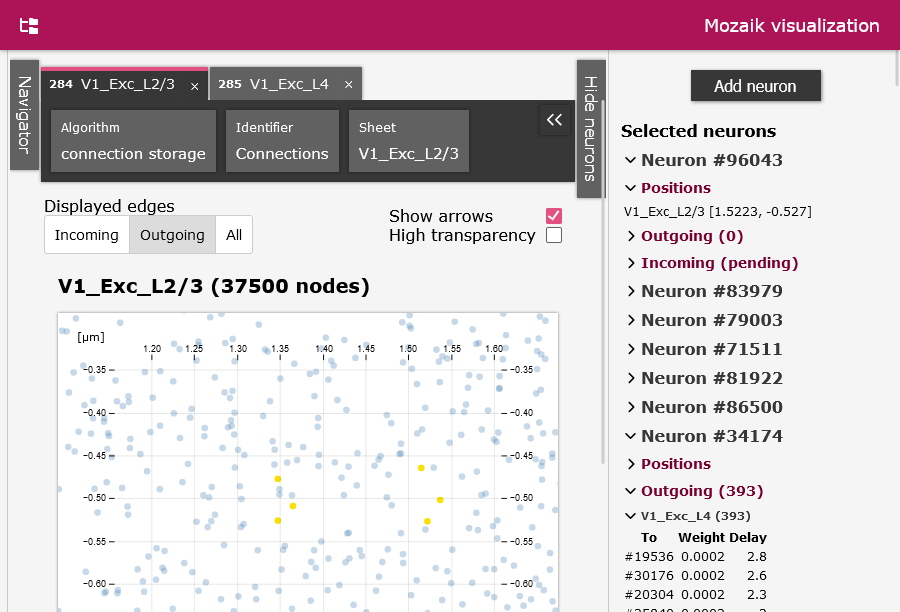
\includegraphics[width=1\linewidth]{img/screenshot_selected_neurons.png}
	\caption{Když jsou vybrané nějaké neurony, vypisují se ve speciální sekci. Vstupní spojení se spočítají až po rozbalení, protože jde o náročnou operaci. Při najetí myší na libovolný neuron se neuron zvýrazní na všech místech, kde je vidět, včetně grafu.}
	\label{fig:selected_neurons}
\end{figure}

\begin{figure}
	\centering
	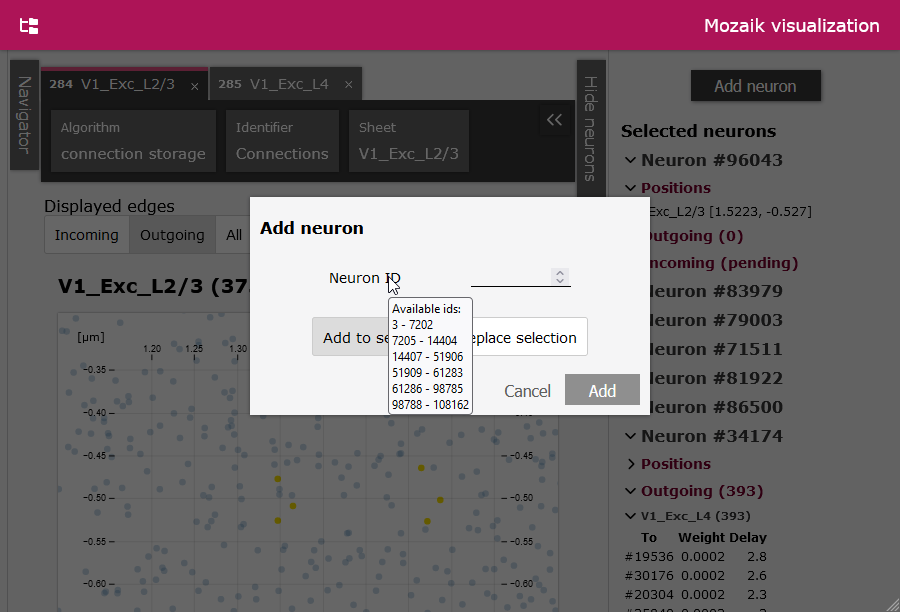
\includegraphics[width=1\linewidth]{img/screenshot_add_neuron.png}
	\caption{Neurony lze vybírat buď v grafech, nebo v tabulce spojení vypsané v sekci vybraných neuronů, nebo pomocí dialogu.}
	\label{fig:add_neuron}
\end{figure}

\begin{figure}
	\centering
	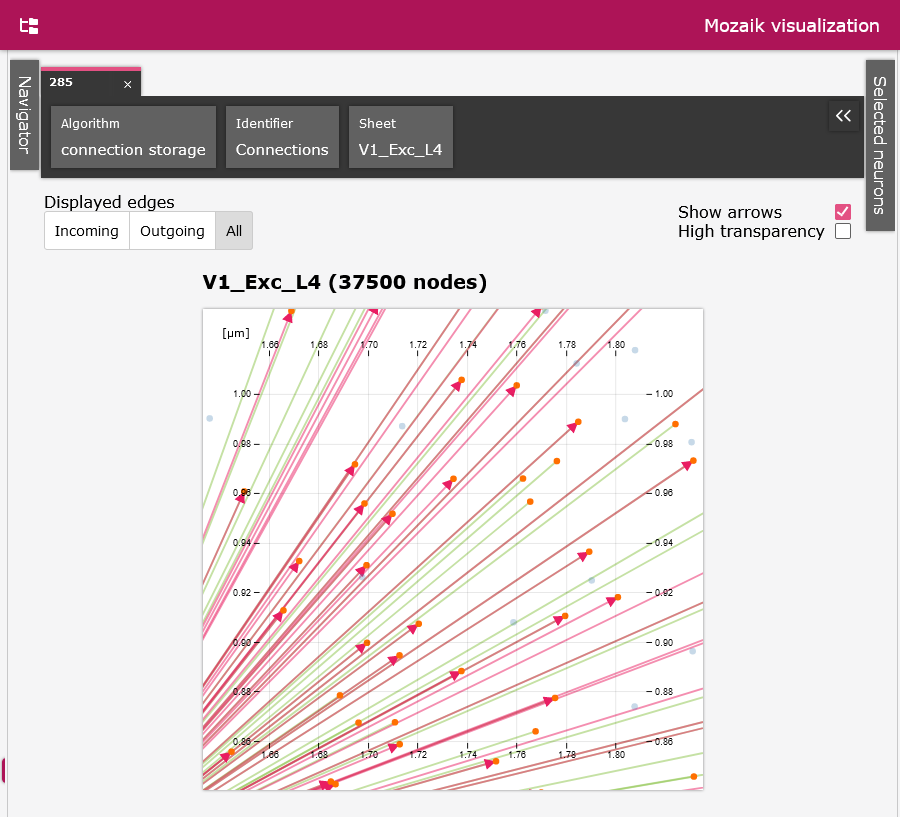
\includegraphics[width=1\linewidth]{img/screenshot_connections.png}
	\caption{Takto vypadá vizualizace spojení v neuronové vrstvě. Červené šipky vedou ven z vybraného neuronu a zelené dovnitř.}
	\label{fig:connections}
\end{figure}

\begin{figure}
	\centering
	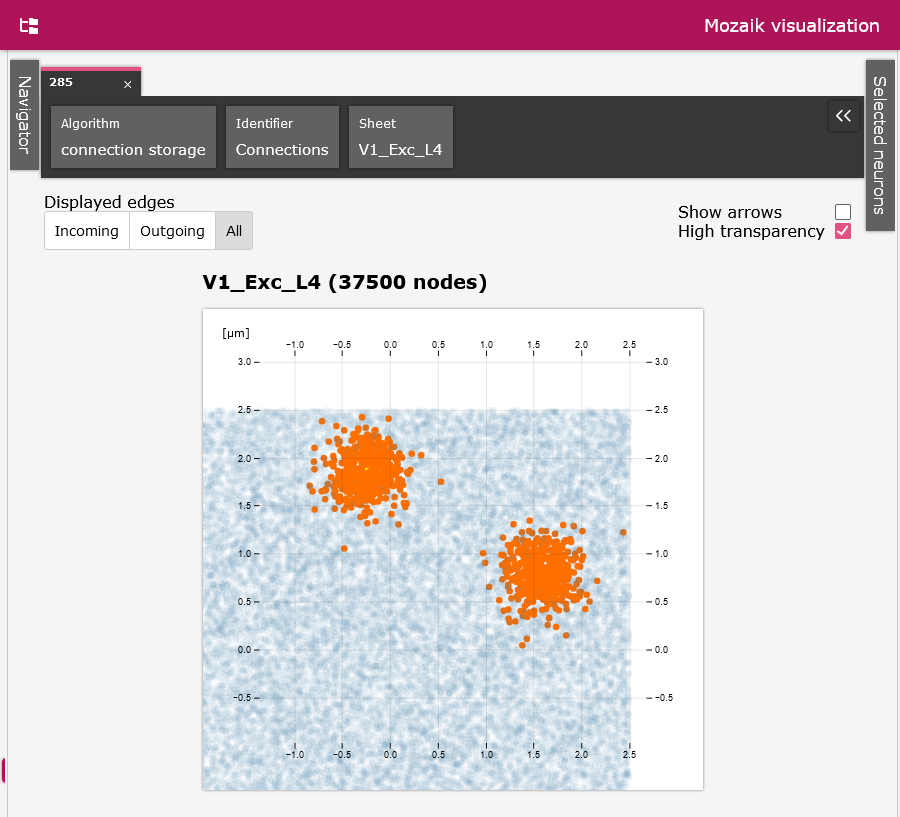
\includegraphics[width=1\linewidth]{img/screenshot_connections_dense.png}
	\caption{Když je neuronů příliš mnoho, spojení jsou špatně vidět. V nastavení vizualizace lze vypnout šipky mezi neurony a zvýšit průhlednost nevybraným.}
	\label{fig:connections_dense}
\end{figure}

\begin{figure}
	\centering
	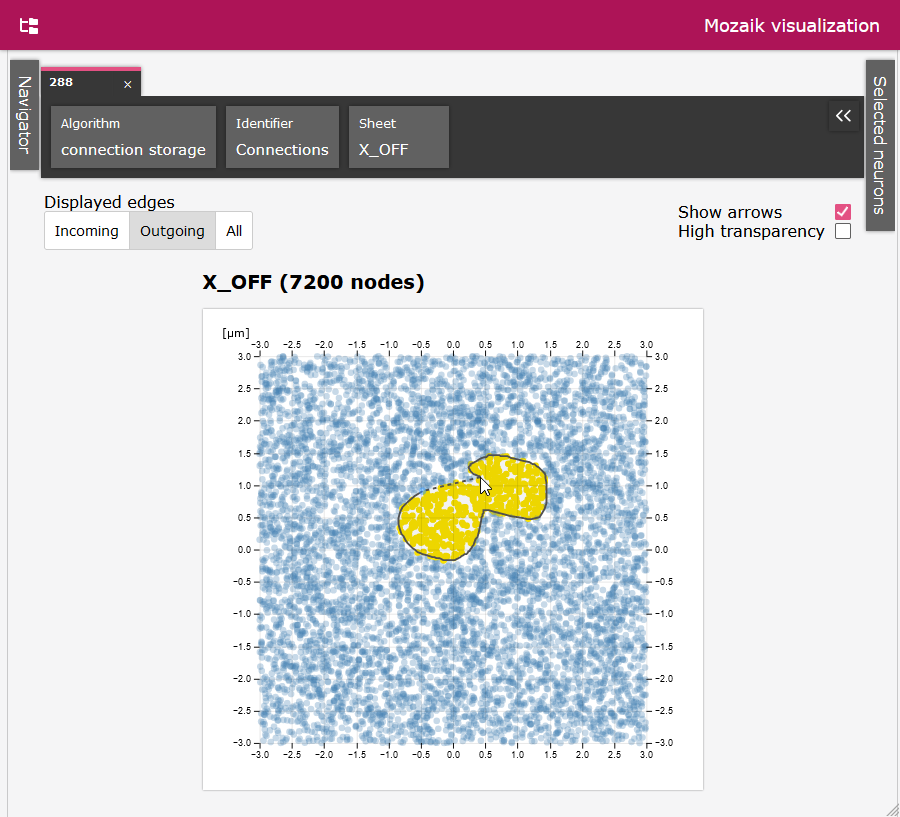
\includegraphics[width=1\linewidth]{img/screenshot_lasso.png}
	\caption{Neuron lze vybrat kliknutím. Kliknutí s klávesou shift neuron do výběru přidá nebo odebere, zachovávajíc ostatní vybrané neurony. Je také možné s klávesou shift opsat myší cestu a vybrat všechny neurony uvnitř. Klávesou escape se pak výběr zruší.}
	\label{fig:lasso}
\end{figure}

\begin{figure}
	\centering
	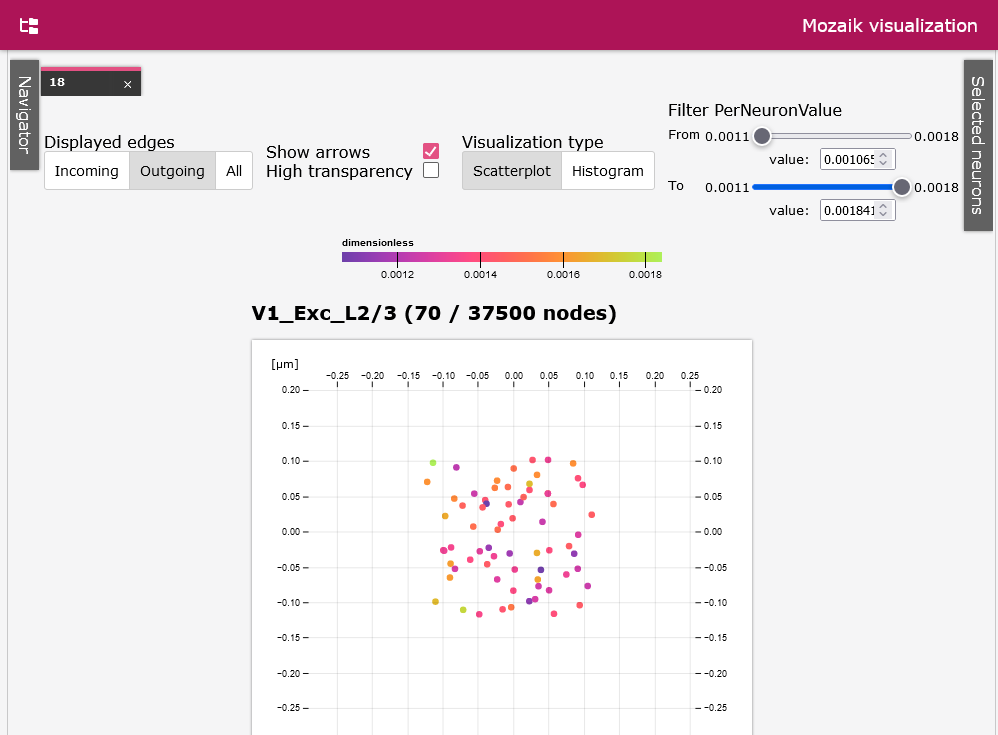
\includegraphics[width=1\linewidth]{img/screenshot_pnv.png}
	\caption{PerNeuronValue ADS je vizualizovaná jako obarvený graf neuronové vrstvy. Kdyby šlo o periodickou veličinu, barevná škála by byla cyklická. Je možné filtrovat neurony na základě jejich hodnoty.}
	\label{fig:pnv}
\end{figure}

\begin{figure}
	\centering
	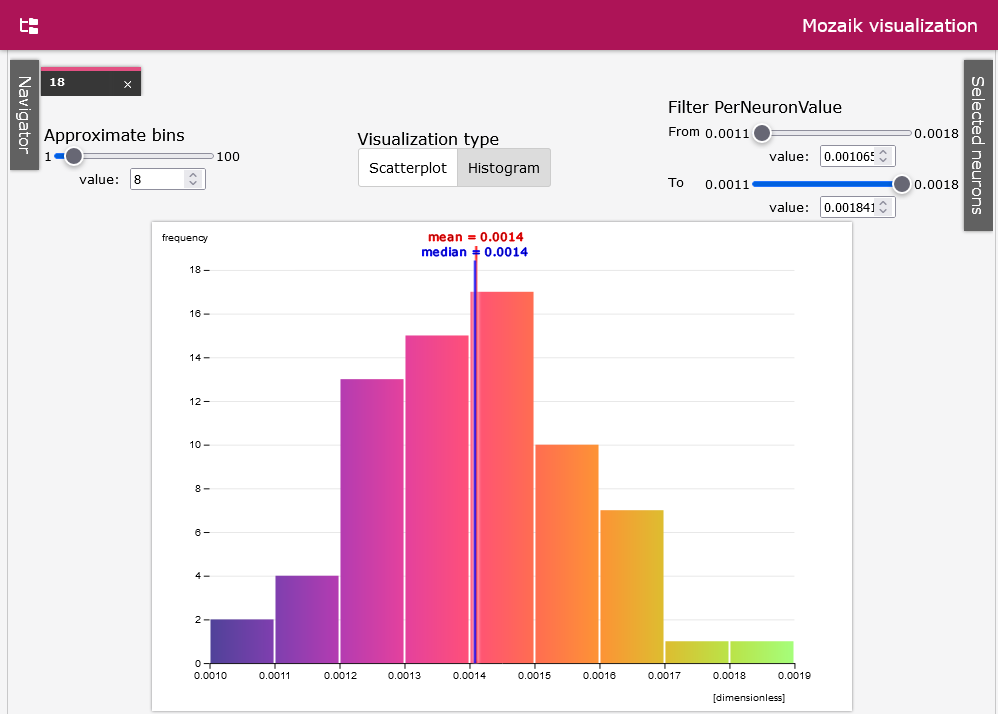
\includegraphics[width=1\linewidth]{img/screenshot_pnv_histogram.png}
	\caption{Alternativní zobrazení PerNeuronValue je v podobě histogramu. Je možné do určité míry ovlivnit počet přihrádek pomocí slideru nahoře vlevo. Histogram ukazuje také medián a aritmetický průměr hodnot.}
	\label{fig:pnv_histogram}
\end{figure}

\begin{figure}
	\centering
	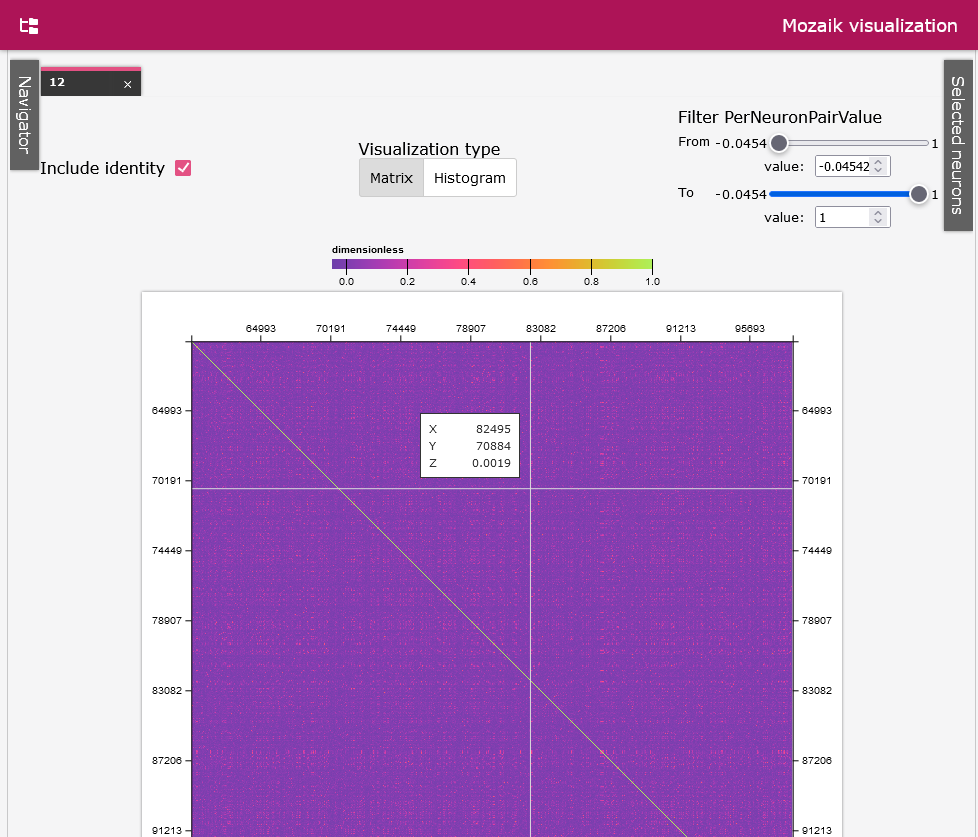
\includegraphics[width=1\linewidth]{img/screenshot_pnpv.png}
	\caption{PerNeuronPairValue je vizualizovaná jako matice. Je možné v ní podobně jako v PerNeuronValue filtrovat hodnoty, stejně tak lze nakreslit histogram. Ten je stejný jako v \ref{fig:pnv_histogram}.}
	\label{fig:pnpv}
\end{figure}

\begin{figure}
	\centering
	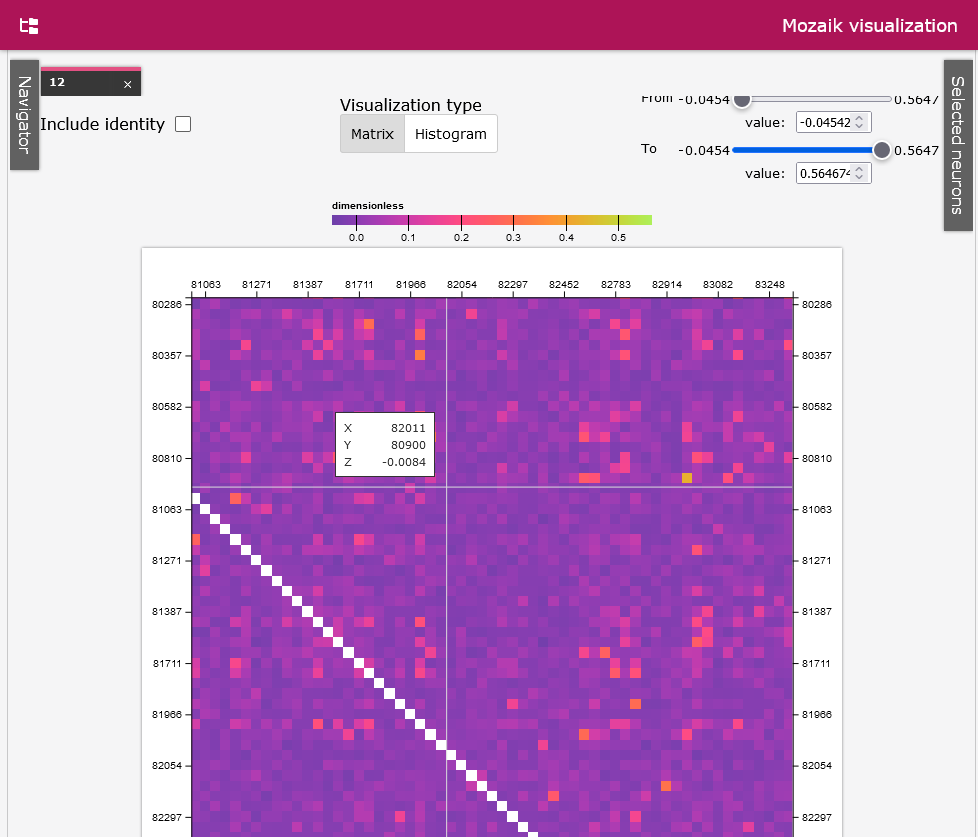
\includegraphics[width=1\linewidth]{img/screenshot_pnpv_noident.png}
	\caption{Jak bylo vidět na obrázku \ref{fig:pnpv}, občas může být na hlavní úhlopříčce hodnota, která výrazně vybočuje z ostatních. Tuto hodnotu je možné vyfiltrovat a zlepšit barevné rozložení.}
	\label{fig:pnpv_noident}
\end{figure}

\begin{figure}
	\centering
	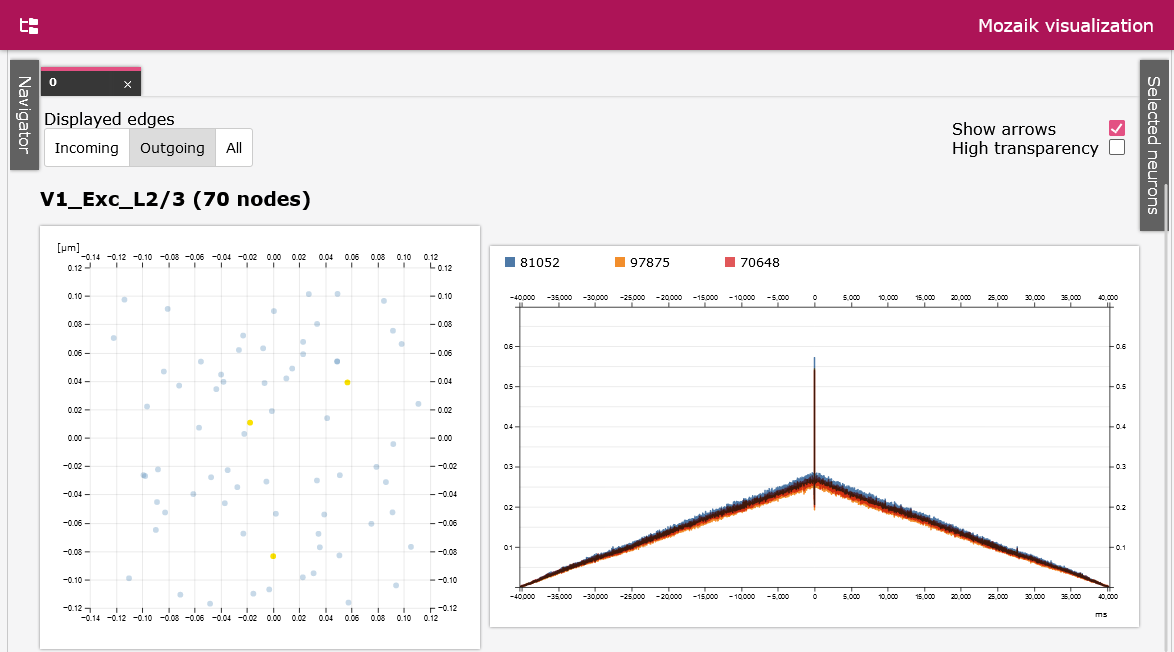
\includegraphics[width=1\linewidth]{img/screenshot_asl.png}
	\caption{AnalogSignalList je zobrazená jako graf neuronů a graf seznamů pro vybrané z nich.}
	\label{fig:asl}
\end{figure}

\begin{figure}
	\centering
	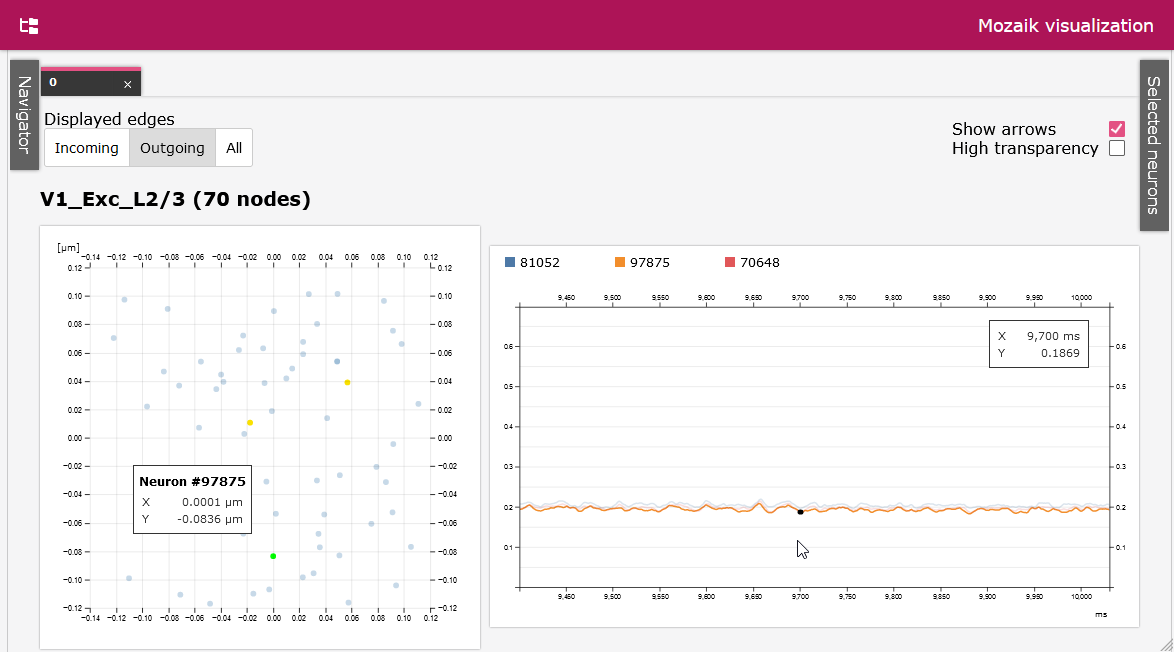
\includegraphics[width=1\linewidth]{img/screenshot_asl_zoom.png}
	\caption{Čárový graf lze zvětšovat podle osy X. Při pohybu myší se zvýrazní nejbližší bod grafu, jeho lomená čára a dotyčný neuron.}
	\label{fig:asl_zoom}
\end{figure}
\chapter{Dokumentace API}
\label{app:api}

\textit{
  Tato dokumentace byla vygenerována z popisu API v souboru \lstinline|/docs/openapi.json|
}

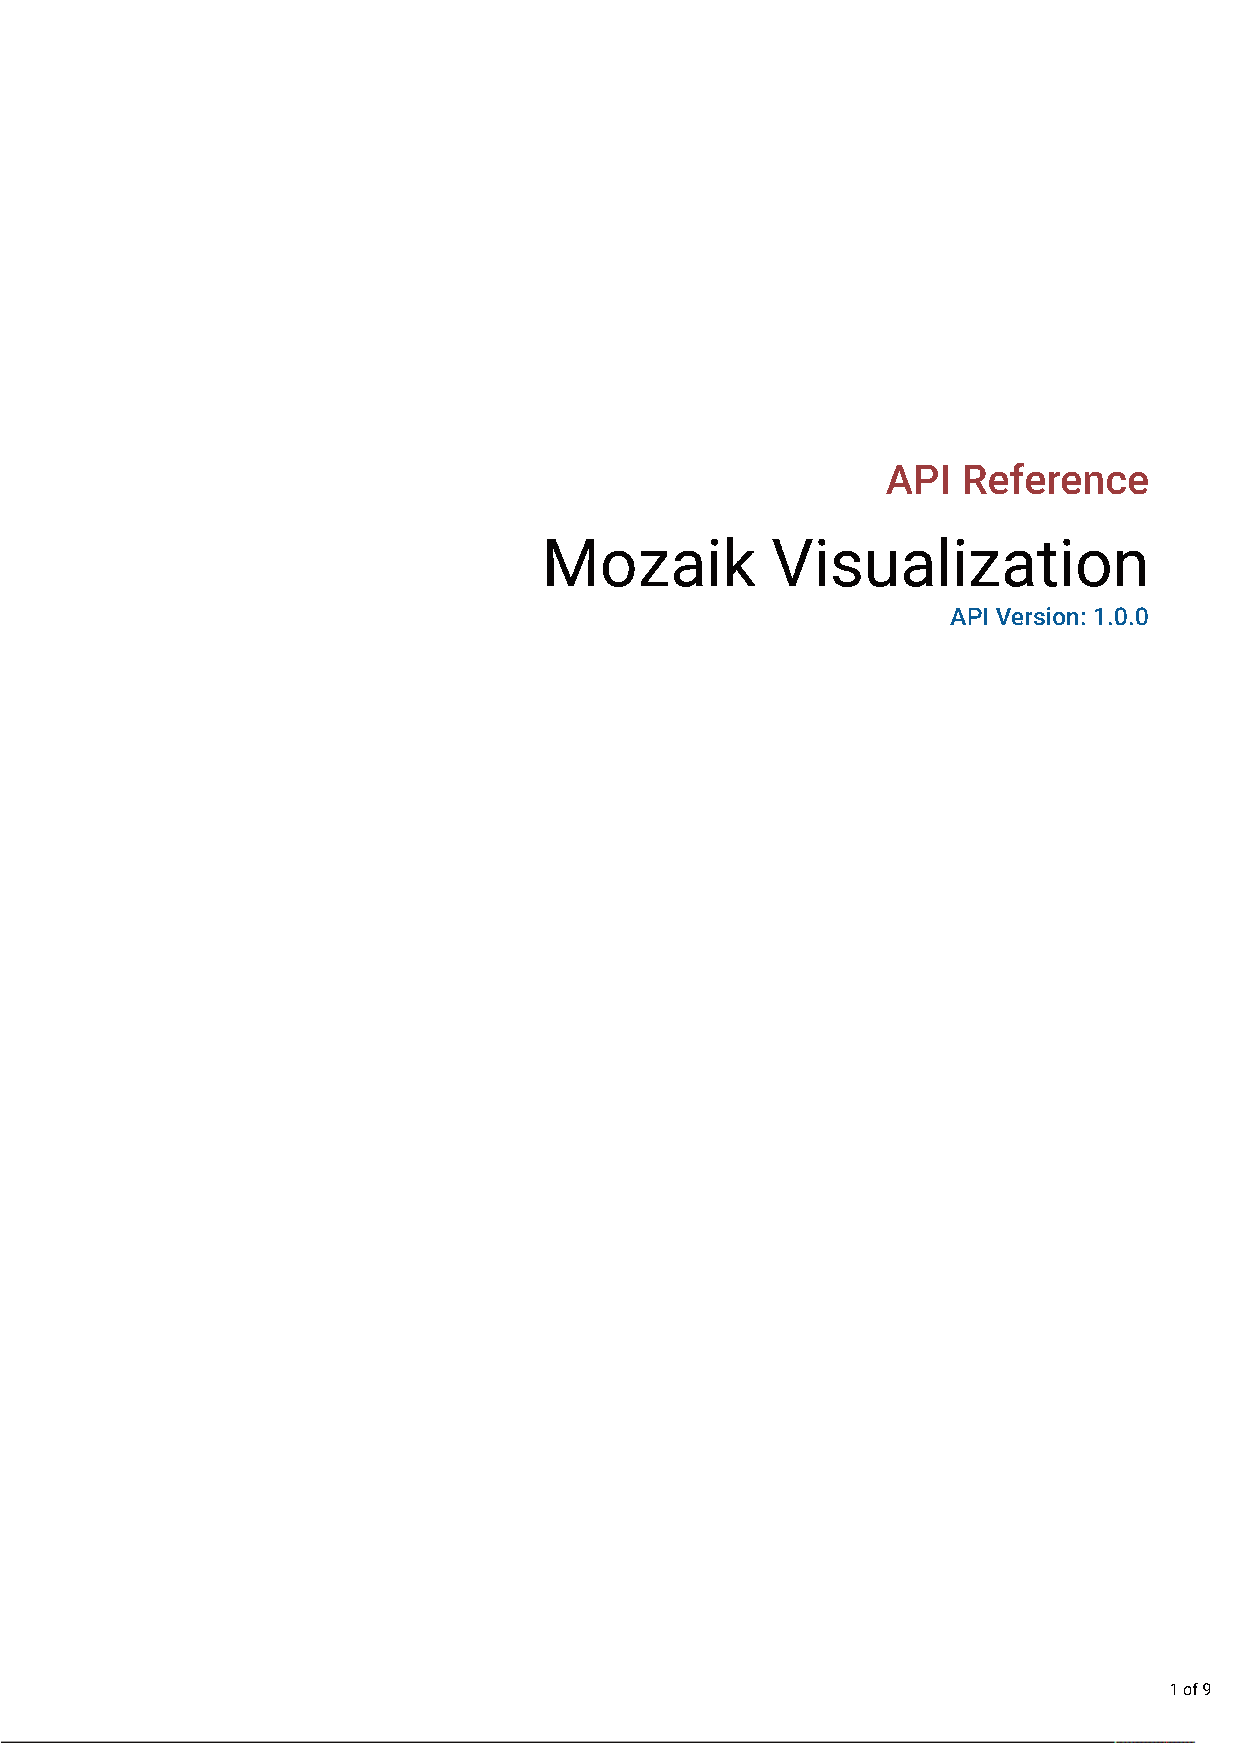
\includepdf[pages=-]{appendices/openapi.pdf}

% if your attachments are complicated, describe them in a separate appendix
%\include{attachments}

\openright
\end{document}
